% Copyright (c) 2005-2009 Center for Urban Simulation and Policy Analysis,
% University of Washington.  Permission is granted to copy, distribute and/or
% modify this document under the terms of the GNU Free Documentation License,
% Version 1.2 or any later version published by the Free Software Foundation;
% with no Invariant Sections, no Front-Cover Texts, and no Back-Cover Texts.
% A copy of the license is included in the section entitled "GNU Free
% Documentation License".

% This is the root latex source file for the Opus and UrbanSim Users Guide.
% The guide is organized as a set of 'include' files, normally one file
% per chapter.  It uses the Python latex documentation standards and latex
% definition files -- see http://www.python.org/doc/current/doc/doc.html
% Also see the "Writing Documentation" chapter in this manual for more
% information.

% Each latex source file (including the 'include' files) should have
% the GNU Free Documentation License as a comment.

\documentclass{latex_files/manual}
\usepackage{amsmath, graphics, graphicx, subfigure,
latex_files/rotating, latex_files/html, upquote, makeidx}
\usepackage{color, latex_files/fancyhdr, longtable, epsfig,lscape,
booktabs,multirow, latex_files/boxit, listings}
% this package causes the font encodings to include an _ (underscore)
% character -- this is useful because then searching the pdf document
% finds names with underscores in them.  (Otherwise the underscore is
% produced using a rule rather than a character and won't show up in
% searches.)
\usepackage[T1]{fontenc}
%\usepackage[ps2pdf]{hyperref}

\sloppy
\newcommand{\tight}{\itemsep 0pt}
\newcommand{\squishlist}{
   \begin{list}{$\bullet$}
    { \setlength{\itemsep}{0pt}      \setlength{\parsep}{3pt}
      \setlength{\topsep}{3pt}       \setlength{\partopsep}{0pt}
      \setlength{\leftmargin}{1.5em} \setlength{\labelwidth}{1em}
      \setlength{\labelsep}{0.5em} } }

\newcommand{\squishlisttwo}{
   \begin{list}{$\bullet$}
    { \setlength{\itemsep}{0pt}    \setlength{\parsep}{0pt}
      \setlength{\topsep}{0pt}     \setlength{\partopsep}{0pt}
      \setlength{\leftmargin}{2em} \setlength{\labelwidth}{1.5em}
      \setlength{\labelsep}{0.5em} } }

\newcommand{\squishend}{
    \end{list}  }

\newcommand{\heading}[1]{\setlength{\parskip}{1em}{\noindent\bf{#1}}} 

\title{The Open Platform for Urban Simulation \\
\includegraphics[width=0.5\textwidth]{images/opus-logo.png}\\
{\em and} UrbanSim \\
Version 4.3 \\ 
%\includegraphics[width=0.15\textwidth]{graphics/new-logo-medium.png}
 ~\\ ~\\
Users Guide and Reference Manual\\ ~\\ ~\\ ~\\ ~\\ ~\\}

\author{The UrbanSim Project \\
University of California Berkeley, and\\ 
University of Washington}

%\authoraddress{Center for Urban Simulation and Policy Analysis \\
%University of Washington \\
%Box 353055 \\
%Seattle, Washington 98195 \\

% Put the real email address only in the pdf version (to avoid including
% a spam magnet in the html version).  A mangled version of the address
% (using "info (at) urbansim.org") is included in the html version by
% a parameter to the latex2html command
%begin{latexonly}
%Email: \email{info@urbansim.org} \\
%Web: \url{http://www.urbansim.org}\\
%end{latexonly}

%}

\date{\textsf{\today}}
% replace \today with a real date (\date{April 1, 2000} ...} when this
% manual is ready for release so that reformatting doesn't cause a
% new date to be used.  For now, setting the date to \today during
% early editing makes it easier to handle versions.


% release version; this is used to define the \version macro
% omit the version unless this is a stable release -- for incremental
% versions just let the date identify the version
% \release{1.0.beta1}

% this tells \index to actually write the .idx file
\makeindex

% not (yet) used:
% \makemodindex                 % If this contains a lot of module sections.

\begin{document}

\maketitle

% Copyright (c) 2005-2009 Center for Urban Simulation and Policy Analysis,
% University of Washington.  Permission is granted to copy, distribute and/or
% modify this document under the terms of the GNU Free Documentation License,
% Version 1.2 or any later version published by the Free Software Foundation;
% with no Invariant Sections, no Front-Cover Texts, and no Back-Cover Texts.
% A copy of the license is included in the section entitled "GNU Free
% Documentation License".

Copyright \copyright{} 2005--2009
Center for Urban Simulation and Policy Analysis,
University of Washington.  

Permission is granted to copy, distribute and/or
modify this document under the terms of the GNU Free Documentation License,
Version 1.2 or any later version published by the Free Software Foundation;
with no Invariant Sections, no Front-Cover Texts, and no Back-Cover Texts.
A copy of the license is included in the section entitled ``GNU Free
Documentation License''.


%% $Id: acknowledgements.tex,v 1.1 2006/01/30 21:12:08 pwaddell Exp $

{\bf \large Acknowledgments}

The project described in this report has been funded principally
by the Puget Sound Regional Council. It was also supported by
grants from the National Science Foundation Grants CMS-9818378,
EIA-0121326 and EIA-0090832, which have supported the development
of UrbanSim.

Numerous people have contributed substantially to the development
of this report and the analysis it contains.  In particular, we
wish to acknowledge the support of Mark Simonson and Larry Blain
at the Puget Sound Regional Council, who coordinated the Technical
Advisory Committee. Considerable assistance was also provided by
Kevin Murphy, Jeff Frkonja, Carol Naito, Jerry Harless, Andy
Norton, Kristen Koch, Neil Kilgren, and others at the PSRC.
Members of the Technical Advisory Committee, listed below, were
instrumental in improving the database and providing valuable
feedback in this effort.  At the Center for Urban Simulation and
Policy Analysis, Chris Peak and Peter Caballero carried out much
of the database development effort, with considerable assistance
from Jack Kim, who analyzed non-residential real estate, Kapena
Pflum, who assisted in documentation and in verification of
employment, Liming Wang, who developed scripts for data
processing, Bjorn-Freeman Benson, Rob Duisberg and David Socha,
who developed key software components to facilitate the data
analysis and processing.

{\bf \large Center for Urban Simulation and Policy Analysis}

The Center for Urban Simulation and Policy Analysis (CUSPA) at the
University of Washington brings advanced research and information
technology to bear on complex social, economic, and environmental
problems in metropolitan areas.  CUSPA is committed to the
development and pursuit of an integrated long-term research agenda
to help understand and anticipate the consequences of policy
choices regarding transportation, land use, housing, community and
economic development, and environmental quality, and to enable
more effective development, implementation, and evaluation of
policies. CUSPA is equally committed to making this research
widely accessible to policymakers and communities through the
development of information technology for advanced simulation
modeling, visualization, and decision support to facilitate
informed and democratic community policy decisions that involve
uncertainty, complex interdependencies, and conflicts over values
and strategies.

CUSPA is structured as an interdisciplinary research center at the
University of Washington, drawing together expertise from across
the campus to address common challenges.  It engages in strategic
partnerships with public agencies to facilitate linking research,
application, and education.  In short, CUSPA attempts to bring the
best available research to bear on the most pressing urban and
environmental problems faced by metropolitan regions in the U.S.
and elsewhere.

\begin{tabbing}
Director: Director: Director: \= \kill Director:\> Paul Waddell,
Evans School of Public Affairs \\
Associate Director:\> Alan Borning, Computer Science and Engineering \\
Steering Committee:\> Marina Alberti, Urban Design and Planning \\
               \> Batya Friedman, Information School \\
\>Scott Rutherford, Civil and Environmental Engineering \\\\
Center Home Page: \> {\bf www.cuspa.washington.edu} \\
UrbanSim Home Page: \> {\bf www.urbansim.org}
\end{tabbing}

\newpage
{\bf \large Technical Advisory Committee} \\

Travis Black -- Kitsap County \\
Larry Blain -- Puget Sound Regional Council\\
Dan Cardwell -- Pierce County \\
Greg Cioc -- Kitsap County \\
Steve Cohn -- City of Bellevue \\
Chandler Felt -- King County \\
Lauren Giboney -- Snohomish County \\
Michael Hubner -- The Suburban Cities Association of King County \\
Tim Koss --Snohomish County \\
Kevin Murphy -- Puget Sound Regional Council\\
Scott Murphy -- Kitsap County \\
Carol Naito -- Puget Sound Regional Council\\
Jennifer Pettyjohn -- City of Seattle \\
Shawn Phelps -- Pierce County \\
Jason Rice -- Kitsap County \\
Mark Simonson -- Puget Sound Regional Council\\
Steve Toy -- Snohomish County \\
Lish Whitson -- City of Seattle \\

% The ugly "%begin{latexonly}" pseudo-environment suppresses the table
% of contents for HTML generation.
%
%begin{latexonly}
\tableofcontents
%end{latexonly}

\newcommand{\package}[1]{\index{opus packages!#1@\textit{#1} package} \textit{#1}}


% start the page numbering for the Part I page, so that it matches the
% actual pages (as shown when viewing the pdf file with Acrobat)
\setcounter{page}{7}

%% $Id: overview.tex,v 1.17 2001/08/18 00:56:25 borning Exp $

\section{Overview of the UrbanSim Architecture}
\label{sec:overview}

To simulate an urban region, UrbanSim employs a collection of
interacting \emph{models}, representing different actors and
processes in the urban environment, such as residents, businesses,
land developers, and transportation networks.  Each model encodes
the behavior of agents in the simulation, as well as the objects
they operate upon, such as land parcels and buildings.  Objects
correlate directly with easily-identifiable objects in the real
world, making it easier to reason about their properties and
behaviors.  Agents can be shared across models, as can the objects
they operate upon.  Much more than other urban modeling systems,
the UrbanSim model is very disaggregate and has high data
requirements.  These requirements enable modeling of processes to
be done at a fine level, which allows use of detailed spatial data
in a manner not possible with more aggregate systems.  At the same
time, this makes the design and implementation of the system more
difficult from a software perspective.  Figure \ref{fig:USArch}
illustrates the software architecture of the UrbanSim system.

\begin{figure*}
\center \resizebox{0.75
\textwidth}{!}{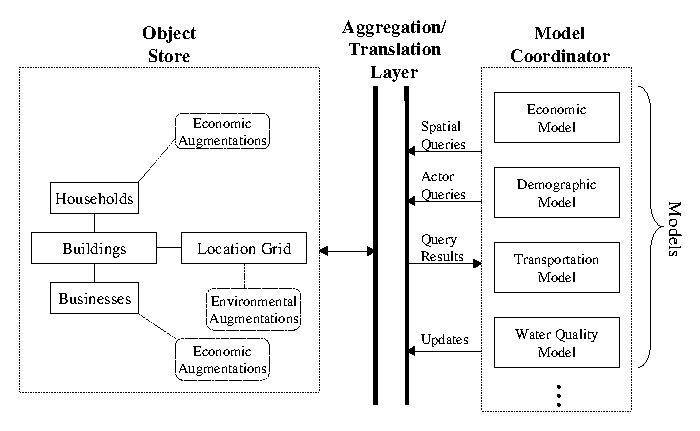
\includegraphics{USDiag1.eps}} \caption{UrbanSim
architecture} \label{fig:USArch}
\end{figure*}

%Figure~\ref{fig:USArch}: UrbanSim architecture.

In addition to the models, the other principal components of
UrbanSim are a \emph{model coordinator} that schedules models to
run and notifies them when data of interest have changed, an
\emph{object store} that holds the shared representations of
agents and other entities in the simulated world, and a
\emph{translation and aggregation layer} that performs a range of
data conversions to mediate between the Object Store and the
models.  The models do not communicate directly with each other;
rather, they communicate via shared data held in the Object Store,
mediated by the translation and aggregation layer.  This
extensible, modular architecture supports system evolution, in
particular replacing a model with a revised one, and creating and
integrating new models.  It allows models to define and share
common sets of objects that they all operate upon, via the Object
Store (regardless of the original source of the data), and also
allows them to monitor changes to data fields, providing a
convenient method for models to synchronize their actions.

A primary goal of this architecture is to move as much of the
software complexity out of the individual models and into the
supporting infrastructure as possible.  This supporting
infrastructure need be written just once, and can have the
attention of an expert programmer.  The models, on the other hand,
are both numerous and frequently changing due to rapidly evolving
theory, methods and modeling needs. Often, specifying them is
difficult, requiring considerable domain-specific expertise,
specialized data, and testing; the more one can relieve the model
designers of programming burdens the better, so that they can
concentrate on issues arising from the domain.

% LocalWords:  Exp UrbanSim USDiag eps noth borning pwaddell

\input{part-gui/gui}
\input{part-components/components}
\input{part-projects/projects}
%% Copyright (c) 2005-2009 Center for Urban Simulation and Policy Analysis,
% University of Washington.  Permission is granted to copy, distribute and/or
% modify this document under the terms of the GNU Free Documentation License,
% Version 1.2 or any later version published by the Free Software Foundation;
% with no Invariant Sections, no Front-Cover Texts, and no Back-Cover Texts.
% A copy of the license is included in the section entitled "GNU Free
% Documentation License".

% This is the root latex source file for the Opus and UrbanSim Users Guide.
% The guide is organized as a set of 'include' files, normally one file
% per chapter.  It uses the Python latex documentation standards and latex
% definition files -- see http://www.python.org/doc/current/doc/doc.html
% Also see the "Writing Documentation" chapter in this manual for more
% information.


\part{Model System Architectures}\label{part-model-system}

\chapter{Sample UrbanSim Projects}

To facilitate learning how UrbanSim works, sample projects and data have been made available for download and use.  Note that these are not in any way operational, but are for demonstration purposes only.  A zone-based sample application is in development, and will be added once it is complete.

\section{Eugene Gridcell Project}

Project name: eugene-gridcell-default

The Eugene Gridcell project is one of the two initial sample projects that are available.  It is based on data compiled by the Lane Council of Governments, and approximates conditions in 1980 for the Eugene-Springfield, Oregon metropolitan area.  The project is an example of an UrbanSim application of the first generation, using gridcells as the unit of geography, with 150 by 150 meter resolution.  The models were developed as part of the development of the initial prototype of UrbanSim approximately during 1996 - 1998.  Many of the models have been modified extensively since that time, for example, as shown in the Seattle-parcel project.

The Eugene gridcell project can be loaded in the GUI, and a baseline simulation can be run using the models as specified previously.  At this time the specification of the models has not been added into the GUI, and therefore the models cannot easily be re-specified or estimated within the GUI.  As time permits, this will be added for demonstration purposes. 

The main advantage and use of the Eugene project is that it is small and runs quickly, so it provides a quick means to test an installation of OPUS and UrbanSim by running a simulation.  Note that little time or effort has been available to fine tune the Eugene application, and the specifications and coefficients are from the initial calibration of the model using a base year of 1994.  So one should not rely heavily on the results, but use the project as intended: a simple demonstration.  It also can be of some use for exploring the data used in the gridcell-based applications.  

\section{Seattle Parcel Project}

Project name: seattle-parcel-default

Recent developments in UrbanSim have included the development of substantial flexibility in the use of geographic units of analysis.  A new model system has been developed for the Puget Sound Regional Council (PSRC), and the previous version of UrbanSim based on gridcells (like the Eugene application) has been converted to use parcels and buildings.  The Seattle parcel project has been generated as a second example project, by taking a snapshot of the PSRC model system and data, and extracting a subset of the database containing only information within the City of Seattle.  In addition, the employment data, which in the PSRC application is confidential, has been replaced with synthetic employment data derived from County Business Patterns by Zip Code for use in the Seattle parcel project.

The main objective in making the Seattle parcel project available to the user community is the same as the original sample project: to make the models and data available for examination by users that may wish to create an application based on the configuration of this project.  Note that the simulation results are not likely to be robust, since the original specifications were from the calibration of the model on the full Puget Sound four county region.

One last caveat for this project: the specifications included in the GUI for models that can be estimated are simply place-holders, and allow a user to experiment with specifying and estimating models in the GUI.  Note that specifying and estimating models in the GUI, if the save results flag is set to true, will overwrite stored specifications and modify simulation results.  This is not a significant concern since this is a sample, experimental project, and not for production use.
\emph{This part under construction...}

three design dimensions (geographic level, degree of aggregation of agents, temporal dimensions); data required for each
%\input{part-model-system/common-data}
% Copyright (c) 2005-2009 Center for Urban Simulation and Policy Analysis,
% University of Washington.  Permission is granted to copy, distribute and/or
% modify this document under the terms of the GNU Free Documentation License,
% Version 1.2 or any later version published by the Free Software Foundation;
% with no Invariant Sections, no Front-Cover Texts, and no Back-Cover Texts.
% A copy of the license is included in the section entitled "GNU Free
% Documentation License".

\chapter{UrbanSim Database Tables}
\label{chapter:urbansim-database-tables}

\emph{\Large Note: This section does not yet represent UrbanSim 4.}

This chapter describes what UrbanSim needs in its baseyear database, ways in
which the baseyear may be structured, how to create a set of scenario databases
that share much of their data, and the use of output databases.

UrbanSim currently uses three types of databases, each of which is described in
more details in following sections:

\begin{description}
\item[baseyear database] -- defining the initial state of a simulation in a
particular base year.
\item[scenario database] -- defining changes to a baseyear (or another scenario)
database.
\item[output database] -- optional repository for simulation results.
\end{description}

\section{Input Database Design: Baseyear and Scenario Databases}
\label{urbansim-database-tables-baseyear-scenario-db}

UrbanSim gets its input data from either a \emph{baseyear} database or a
\emph{scenario} database.  The UrbanSim simulator treats \emph{baseyear} and
\emph{scenario} databases as read-only databases, however other data
preparation applications such as the estimators or the household synthesizer
may write to them.  In fact, when the run manager starts a new simulation, the
first step is to copy the baseyear data into the baseyear cache. The
simulation then reads all of its baseyear information from the baseyear cache
and writes all results to the simulation cache. \simulationcacheindex Data is only written to the
output database when specified (currently done manually).

At the moment, UrbanSim only supports the MySQL \mysqlindex database server (we will be
adding support for other database servers).

A \emph{baseyear} database contains a snapshot of the base
information defining the initial state before the UrbanSim
simulation. Most of the data typically is about a particular year,
e.g., geographic information, initial household and job information,
etc., for a given year.

A \emph{scenario} database contains additional and augmenting information to
alter the base year data when simulating a particular scenario e.g., new
transportation links, an expanded urban growth boundary, etc. Any of the table
may be placed in either of the database, although typically most are placed in
the baseyear database.  The scenario databases typically only contains tables
specifying different possible futures, e.g. tables of exogenous events
scheduled for future years.

The way that the scenario can modify the information in the baseyear database or
another scenario database is determined by the scenario linking.

\subsection{Scenario Linking}

The scenario databases are linked to each other and, eventually, to a baseyear
database via a tree structure: each scenario can refer to exactly one parent
database; that parent can be either another scenario or a baseyear database.
The baseyear database is the root of the tree.  In this way, multiple scenarios
may share the same baseyear.

When UrbanSim looks for a particular input database table, it traverses this
chain looking for that table.  The first table matching that name is used.  In
this way, any tables contained in the scenario database ``shadow'' or ``hide''
the same-named tables in the scenario's parent database(s).

Consider these example of how to create derivative scenarios:\\

\begin{center}
\includegraphics*{scenarios}
\end{center}

\begin{itemize}
\item Scenario 1 is the base year plus a larger urban growth boundary, thus
scenario 1's parent is the base year database. The UrbanSim scenario file will
specify the scenario 1 database as the ``scenario-data''.
\item Scenario 2 is the base year plus a major employer leaving the
municipality. Scenario 2's parent is also the base year database. The UrbanSim
scenario file will specify the scenario 2 database as the ``scenario-data''.
\item Scenario 3 is the same as scenario 1, but with additional changes in the
zoning laws to compensate for the larger UGB. Scenario 3's parent is scenario 1
and the UrbanSim scenario file will specify the scenario 3 database as the
``scenario-data''.
\item Scenario 4 is the same as scenario 1, but with changes in the population
demographics as a result of the larger UGB. Scenario 4's parent is scenario 1
and the UrbanSim scenario file will specify the scenario 4 database as the
``scenario-data''.
\end{itemize}

Any table in a scenario database ``hides'' the same-named table in the
scenario's parent database.

\subsection{Scenario Database Design}

The only required table in the scenario database is the
\verb|scenario_information| table (see Sec.~\ref{urbansim-database-tables-scenario-inforamtion}).
This table points to its parent, i.e. to a baseyear database, or
to another scenario database.

In addition, the scenario database may include any other tables for data that
is different in this scenario. For example, if the scenario is simulating a
large retail development in the suburbs, the \verb|development_events_exogenous| table
would be included in the scenario database.  In this way, a scenario database
may change any of the information contained in the baseyear.

\section{Output Database}

An output database may contain the results of an UrbanSim simulation.  This
database is optional; the urbansim cache is the primary storage location for
simulation inputs and results.

\section{General Database Design}

\subsection{Guidelines}

Here are some guidelines on database design:

\begin{itemize}
\item Use only lower-case letters, digits, and underscores for the names of
databases, database tables, and database columns. This avoids problems when
moving database between different operating systems (e.g. between Windows \windowsindex and
Linux). \linuxindex
\item Avoid overly abbreviated names.  While very short names were required by
some other systems, UrbanSim itself has no limit on the length of names. Most
database system allow database names, table names and column names to be 32
characters, 64 characters (e.g. MySQL), \mysqlindex or more.
\end{itemize}

\subsection{Data Types}

\index{Python!data types} \index{Opus!data types} \index{MySQL!data
types} When Opus reads data from a database table, it stores the
data in a Python type that is close to the type of the corresponding
column in the database.  The particular mapping between database
types and Python types currently is defined for MySQL \mysqlindex
and should be re-defined for each additional type of database.  The
conversion for MySQL is:

\begin{tabular}{ll}
MySQLdb FIELD_TYPE & Python/numpy type \\
\hline
tinyint(1) & bool8 \\
short & int16 \\
int24 & int32 \\
long & int32 \\
longlong & int64 \\
float & float32 \\
double & float64 \\
decimal & float64 \\
\end{tabular}

Similarly, when writing from Python to a database, Opus converts from Python
types to database-specific data types.  The conversion for MySQL is:

\begin{tabular}{ll}
Python/numpy type & MySQL type \\
\hline
bool8 & int(1) \\
int8 & int(8) \\
int16 & int(16) \\
int32 & int(32) \\
int64 & int(64) \\
float32 & float \\
float64 & double \\
\end{tabular}

Note that these conversions are not symmetrical, since multiple
database types map onto a single Python type.  The result is that
when written back to the database, the column types may change from
that of the input database table.

\section{What Tables are Used in UrbanSim?}
%
Most database tables are optional. The required set of tables is determined by the set of models configured for
a run. Details can be found in the description of the particular models in Section~\ref{sec:urbansim-models}. 

Additionally, some tables and various attributes of tables are determined by 
the variables used by the models.  This can be found by looking at the models'
specification tables.

The \verb|tables_to_cache| argument of
\verb|urbansim.configs.cache_baseyear_configuration| lists the tables required for the standard set of models 
in a production run of UrbanSim. Additional tables can be used in post-processing, for example for creating
indicators.


\section{Coefficients and Specification Tables}

The UrbanSim models are configured through user specified
variables and coefficients. The coefficients should be
estimated separately for each region to be modeled by UrbanSim. The art and
science of estimating the coefficients is a matter for a series of college
courses so this description assumes that appropriate variables for each model
have been chosen, and the appropriate coefficients have been estimated for
those variables.

Each of the regression models and Logit models have two associated
tables: a table to store the specification of what variables to use
for that model, and a table to store the estimated coefficients to
use for those variables.  The names of these tables are composed by
appending either \verb|_coefficients| or \verb|_specification| to
the model name.  The tables for the land price model, for instance,
are \verb|land_price_model_coefficients| and
\verb|land_price_model_specification|.

All coefficient tables share the same schema, as do all
specification tables. The schemas are:


\subsection{Specification table}

\begin{tabular}{|l|l|p{4.5in}|}

\hline
\textbf{Column Name} & \textbf{Data Type} & \textbf{Description} \\\hline 
variable_name & varchar & A legitimate specification for an Opus variable (see below).\\\hline 
coefficient_name & varchar & Name of a coefficient connected to this variable.\\\hline
sub_model_id & integer & \emph{(optional)} Defines the submodel, if the model
contains submodels. If the model does not have multiple submodels, use ``-2'' for this field, or leave it out.\\\hline
equation_id & integer & \emph{(optional)} If a submodel has multiple equations, this field
contains an id identifying which equation this row applies to.  If a model does
not have multiple equations, use ``-2'' for this field, or leave it out. \\\hline
fixed_value & double & \emph{(optional)} If a coefficient should have a fixed value for an estimation,
it should be set in this column. All values that are not equal to 0 are considered as fixed values.\\
\hline
\end{tabular}

\begin{itemize} \tight
\item Values of the sub_model_id column are
determined by the \verb|submodel_string| parameter of the model, see e.g. initialization of \class{ChoiceModel} 
(\ref{sec:choice-model})
or \class{RegressionModel} (\ref{sec:regression-model}). Specifically, the values of the sub_model_id column must 
exist in the \verb|submodel_string| attribute of the model's dataset.
The employment location choice models, for instance, define submodels by
employment sectors, so the values of this field are the
\verb|sector_id| values
of the jobs dataset. 
\item Each combination of (sub_model_id, coefficient_name)
must exist in the model's coefficients table.
\item Each combination of (sub_model_id, equation_id, variable_name) must be unique.
\item If fixed_value is non-zero in at least one row of the table, set the remaining values to 0. Currently, fixed_value 
are considered only in the estimation of \class{ChoiceModel}.
\item Specific models have additional requirements: see Developer Model and Non-home-based Employment Location Choice Model. 
\end{itemize}

A legitimate specification for an Opus variable may be one of the following:

\begin{itemize}

\item The word \verb|constant| indicating a value specific to this combination
of (sub_model_id, equation_id).

\item The name of a primary attribute of a dataset, specified as a period-separated
tuple of dataset name, attribute name, .e.g.
\verb|gridcell.percent_slope|.

\item The name of a dataset attribute, specified as a period-separated triple of
Opus package name, dataset name, attribute name, .e.g. \verb|urbansim.gridcell.population|.

\item Any Opus expression as described in~\ref{chapter:expressions}.
 
\item Any word preceeded by '__' will be considered as a special parameter without a relation to an Opus variable.
It can be used for estimating additional parameters.
\end{itemize}

\subsection{Coefficient table}

\begin{tabular}{|l|l|p{4.5in}|}

\hline
\textbf{Column Name} & \textbf{Data Type} & \textbf{Description} \\

\hline
coefficient_name & varchar & Unique name of a coefficient  \\

\hline
estimate & double & The estimated value of this coefficient \\

\hline
sub_model_id & integer &  \emph{(optional)} Identifier for a submodel, or
-2 if not used. \\

\hline
standard_error & double & \emph{(optional) }
The standard error of this estimated value. This is for reference only and is
not used by UrbanSim.  \\

\hline
t_statistic & double & \emph{(optional) }
The t-statistic of this coefficient for the test of significance from 0. This
is for reference only and is not used by UrbanSim.  \\

\hline p_value & double & \emph{(optional) } The p-value of this t-statistic,
gives the Prob(|x|\textgreater{}|estimated coefficient|) when x is drawn from a
t-distribution with mean 0. This is for reference only and is not used by
UrbanSim.   \\

\hline

\end{tabular}

\begin{itemize} \tight
\item Each combination of (sub_model_id, coefficient_name) must be unique and must exist in the model's specification table.
\end{itemize}

\section{Database Tables about Development Types}
\label{sec:development-tables}

\emph{Development types} are used to classify a grid cell according to the
``type'' of development currently in the grid cell.  For instance, grid cells
with only a few residential units and no other square footage might be
classified as ``low density residential'' which may be abbreviated as ``R1''.
Other grid cells may be classified as mixed use, commercial, etc.  The set of
development types to use is arbitrary.

Development types are grouped by two nested mechanisms: \emph{groups} and
\emph{non-overlapping-groups}. Each development type may be a member of
multiple groups. Each group may be a member of multiple
non-overlapping-groups. All of the groups in a non-overlapping-group must be
disjoint (i.e., may not share any development types); in other words, each
development type must belong to at most one group in each
non-overlapping-group.

Groups and non-overlapping-groups are used in the computation of the variables
in the models, so to fully understand them requires understanding the model 
definitions.

\subsection{The {\tt development_types} table}

Each row defines one development type.

\begin{tabular}{|l|l|l|}

\hline
\textbf{Column Name} & \textbf{Data Type} & \textbf{Description} \\

\hline development_type_id & integer & Unique identifier for this row.  \\

\hline name & varchar & Name of the development type.  \\

\hline min_units & integer & Minimum number of units to be in this development
type.  \\

\hline max_units & integer & Maximum number of units to be in this development
type.  \\

\hline min_sqft & integer & Minimum square feet to be in this development type.
\\

\hline max_sqft & integer & Maximum square feet to be in this development type.
\\

\hline

\end{tabular}

\begin{itemize}
\tight
\item development_type_id must be unique and greater than zero. We recommend that it starts at 1 and is sequential.
\item min_units must be \textgreater{}= 0.
\item max_units must be \textgreater{}= min_units.
\item min_sqft must be \textgreater{}= 0.
\item max_sqft must be \textgreater{}= min_sqft.
\item The development types should not overlap, and should completely cover the
space.  A grid cell should only be able to be in a single development type.
\end{itemize}

\subsection{The {\tt development_type_groups} table}
\label{sec:development-tables-type-groups}

Each row defines one development type group, but not the group's
membership - the memberships are defined in the \verb|development_type_group_definitions| table.

\begin{tabular}{|l|l|l|}

\hline
\textbf{Column Name} & \textbf{Data Type} & \textbf{Description} \\

\hline group_id & integer & Unique identifier for this row.  \\

\hline name & varchar & Unique name of the development type group.  \\

\hline non_overlapping_groups & varchar & Name of the non-overlapping-group or
empty for no non-overlapping-group.  \\

\hline
\end{tabular}

\begin{itemize}
\tight
\item group_id must be unique, and greater than zero.
\item name must be unique. The required development type groups must be lower
case with underscores between words e.g. high_density_residential. We recommend
that all names follow this style.
\item names and non_overlapping_groups names must not contain spaces.
\item names and non_overlapping_groups names must be lower-case.
\item Development types must not overlap across the groups in the same
non_overlapping_groups.
\end{itemize}

The set of required development type groups and non-overlapping-groups is
determined by the set of variables used by the models being estimated or
simulated.  Thus, there is no way to a-priori specify which development type
groups will be needed for your application of UrbanSim. There are two exceptions:
First, the model Events Coordinator is internally using groups 'residential', 'mixed_use', 'commercial',
'industrial', and 'governmental'. Second, the Land Price Model (\ref{sec:land-price-model}) is using by default a filter
that requires a group called 'developable'. Therefore, if you do not change this settings, make sure your
table contain these entries.

UrbanSim requires some non-overlapping-groups and requires those to have
certain groups within them, though they may have additional groups as well.

\subsection{The {\tt development_type_group_definitions} table}

This table defines the set of \verb|development_types| in each
development type group. Each row defines one ``belongs to'' relationship (a
particular development type that ``belongs to'' a particular
development type group).

\begin{tabular}{|l|l|l|}
\hline
\textbf{Column Name} & \textbf{Data Type} & \textbf{Description} \\

\hline
development_type_id & integer & Index into the development_types table  \\
\hline
group_id & integer & Index into the \verb|development_type_groups| table  \\
\hline

\end{tabular}

\begin{itemize}
\tight
\item development_type_id must be a valid index into the \verb|development_types| table
\item group_id must be a valid index into the \verb|development_type_groups| table
\item The combination of development_type_id and group_id must be unique

\end{itemize}

\subsection{Example}

Let R1-R3 be in the
``residential'' group in the ``dynamic_land_use_variables''
non-overlapping-group, M4-M5 be in the ``mixed_use'' group in the
``dynamic_land_use_variables'' non-overlapping-group, and C1-C9 be in the
``commercial'' group in the ``dynamic_land_use_variables''
non-overlapping-group. Also let R3 and M5 be in the
``high_density_residential'' group, and ``M5'' and ``C4'' be in the
``noisy_commercial'' group.

This example would involve these two tables: (note: R1=1, R2=2, R3=3,
M4=4, M5=5, C1=6, \ldots, C4=9, etc)

\begin{center}
\begin{tabular}{c}

\begin{tabular}{|l|l|l|}
\multicolumn{3}{c}{\textbf{\tt|development_type_groups|}} \\
\hline
group_id & name & non_overlapping_groups \\

\hline
50 &residential &dynamic_land_use_variables \\

\hline
51 &mixed_user &dynamic_land_use_variables \\

\hline
52 &commercial &dynamic_land_use_variables \\

\hline
100 &high_density_residential & \\

\hline
101 &noisy_commercial & \\

\hline
\end{tabular}

\\ \\

\begin{tabular}{|l|l|}
\multicolumn{2}{c}{\textbf{\tt|development_type_group_definitions|}} \\

\hline
development_type_id & group_id \\

\hline
1 & 50 \\
\hline
2 & 50 \\
\hline
3 & 50 \\
\hline
4 & 51 \\
\hline
5 & 51 \\
\hline
6 & 52 \\
\hline
... &  \\
\hline
3 & 100 \\
\hline
5 & 100 \\
\hline
9 & 101 \\
\hline
5 & 101 \\
\hline
\end{tabular}

\end{tabular}
\end{center}


Note that:
\begin{itemize}
\tight
\item R3 belongs both to groups ``residential'' and
``high_density_residential''.
\item R1 belongs to group ``residential''.
\item M5 belongs to groups ``mixed_use'', ``high_density_residential'', and
``noisy_commericial''.
\end{itemize}


\section{Database Tables about Development Events}
\label{sec:db-tables-events}
These tables represent events in the real estate development. Events that are scheduled 
to take place in the future are stored in the {\tt development_events_exogenous} table,
events that occured prior to the base year are stored in the {\tt development_event_history} table.

Both tables can contain columns of the pattern ``{\it units}_{\tt change_type}''. Each value determines
a type of change for that type of {\it units}. Possible values are:
\begin{itemize} \tight
\item ``A'' for Add
\item ``R'' for Replace
\item ``D'' for Delete
\end{itemize}
If this column is missing for a certain type of units, the default value is ``A'' for all events.

\subsection{The {\tt development_events_exogenous} table}

These development events are changes to grid cells which are scheduled to take
place
in the future. For any given year, it is possible to schedule any number of
changes to the attributes of any number of gridcells. Each change represents
that addition, subtruction or replacement of the specified number of sqft, residential units, and
improvement values.  For example, if
GridCell 23 is to grow by 200 residential units in 2008 (an apartment building
is built), the table would include a row with scheduled_year = 2008, grid_id =
23, residential_units = 200, and residential_units_change_type = 'A'.

The value in the ``improvement_value'' fields, below, are used to indicate how
to change the associated improvement_value for this grid cell. Each event will
add/subtract/replace (improvement_value * (number
of units [or sqft] being built by this event)) to the current improvement value
in
this grid cell.  The units of the improvement is currency value, e.g. dollars.

\begin{tabular}{|p{2in}|l|p{3.5in}|}
\hline
\textbf{Column Name} & \textbf{Data Type} & \textbf{Description} \\
\hline
grid_id & integer & Grid cell where the event takes place  \\
\hline
scheduled_year &short & Year in which the event will be implemented  \\
\hline
starting_development_type_id & integer & \emph{(optional) }
This field is ignored. It is here so that the schema is the same for the
\verb|development_events_exogenous| and \verb|development_event_history| tables.   \\
\hline
ending_development_type_id & integer &  This grid cell's development type
at the ending of the scheduled_year. Index into the \verb|development_types|
table   \\
\hline
residential_units & integer & \\
\hline
commercial_sqft & integer & \\
\hline
industrial_sqft & integer & \\
\hline
governmental_sqft & integer & \\
\hline
residential_units_change_type & char & \emph{(optional) } see \ref{sec:db-tables-events}\\
\hline
commercial_sqft_change_type & char & \emph{(optional) } see \ref{sec:db-tables-events}\\
\hline
industrial_sqft_change_type & char & \emph{(optional) } see \ref{sec:db-tables-events}\\
\hline
governmental_sqft_change_type & char & \emph{(optional) } see \ref{sec:db-tables-events}\\
\hline
residential_improvement_value & integer & See description, above  \\
\hline
commercial_improvement_value & integer & See description, above  \\
\hline
industrial_improvement_value & integer & See description, above  \\
\hline
governmental_improvement_value & integer & See description, above  \\
\hline
fraction_residential_land_value & float & Fraction of residential land in this cell  \\
\hline

\end{tabular}

\begin{itemize} \tight
\item fraction_residential_land_value must be between 0 and 1
\item grid_id must be a valid id in the \verb|gridcells| table or zero
\item development_type_id must be a valid index into the \verb|development_types| table or zero
\end{itemize}


\subsection{The {\tt development_event_history} table}
\label{sec:table-development-event-history}

The development event history records the development events that occurred
prior to the base year. It is used by the development project transition model~(\ref{sec:development-project-transition-model}),
and for ``unrolling'' the baseyear to create versions of the gridcell data for
prior years.

This table uses a subset of the schema used for
\verb|development_events_exogenous|.  It
can be considered an extension back in time of the \verb|development_events_exogenous|
table, though with additional constraints, specified below.

\begin{tabular}{|p{2in}|l|p{3.5in}|}
\hline
\textbf{Column Name} & \textbf{Data Type} & \textbf{Description} \\
\hline
grid_id & integer & Grid cell where the event takes place  \\
\hline
scheduled_year &short & Year in which the event was implemented  \\
\hline
starting_development_type_id & integer & \emph{(optional) }
This will be the value of the development_type for this gridcell after
``unrolling'' this development event. \\
\hline
residential_units & integer & \\
\hline
commercial_sqft & integer & \\
\hline
industrial_sqft & integer & \\
\hline
governmental_sqft & integer & \\
\hline
residential_units_change_type & char & \emph{(optional) } see \ref{sec:db-tables-events}\\
\hline
commercial_sqft_change_type & char & \emph{(optional) } see \ref{sec:db-tables-events}\\
\hline
industrial_sqft_change_type & char & \emph{(optional) } see \ref{sec:db-tables-events}\\
\hline
governmental_sqft_change_type & char & \emph{(optional) } see \ref{sec:db-tables-events}\\
\hline
residential_improvement_value & integer & See description, above  \\
\hline
commercial_improvement_value & integer & See description, above  \\
\hline
industrial_improvement_value & integer & See description, above  \\
\hline
governmental_improvement_value & integer & See description, above  \\
\hline

\end{tabular}

\begin{itemize} \tight
\item grid_id must be a valid id in the \verb|gridcells| table or zero
\item development_type_id must be a valid index into the \verb|development_types| table or zero
\end{itemize}

In addition, the following will produce warnings:
\begin{itemize} \tight
\item Warn if scheduled_year is greater than or equal to the base year. Such
entries will not be used.
\end{itemize}

\section{Development Constraints and Target Vacancies}
%
\subsection{The {\tt development_constraints} table}

This table defines rules that restrict the possible development types a
developer can create on a particular grid cell.  Each row defines one rule.
Development is not allowed on any gridcell that matches any of these rules.  A
gridcell matches a rule if the attribute values for the gridcell match all of
the values in the rule (rule columns with the value ``-1'' are ignored when
determining a match).

\begin{tabular}{|l|l|p{3.5in}|}

\hline
\textbf{Column Name} & \textbf{Data Type} & \textbf{Description} \\

\hline constraint_id & integer & Unique rule identification number  \\

\hline \emph{name-of-a-gridcell-attribute} & integer or float &  Value for this
attribute, or ``-1'' if this attribute is not part of the constraint (e.g.
\emph{don't care}) \\

\hline min_units & integer & Minimum number of residential units for a gridcell.
A development project may only be placed on this gridcell if it will result in
this gridcell containing at least this number of residential units. \\

\hline max_units & integer & Maximum number of residential units for a gridcell.
A development project may only be placed on this gridcell if it will result in
this gridcell containing at most this number of residential units. \\

\hline min_commercial_sqft & integer & Minimum number of commercial
sqft. for a gridcell.  A development project may only be placed on
this gridcell if it will
result in this gridcell containing at least this number of commercial sqft. \\

\hline max_commercial_sqft & integer & Maximum number of commercial
sqft. for a gridcell. A development project may only be placed on
this gridcell if it will
result in this gridcell containing at most this number of commercial sqft. \\

\hline min_industrial_sqft & integer & Minimum number of industrial
sqft. for a gridcell.  A development project may only be placed on
this gridcell if it will
result in this gridcell containing at least this number of industrial sqft. \\

\hline max_industrial_sqft & integer & Maximum number of industrial
sqft. for a gridcell. A development project may only be placed on
this gridcell if it will
result in this gridcell containing at most this number of industrial sqft. \\

\hline
\end{tabular}

\begin{itemize}
\tight
\item constraint_id must be a unique positive integer.

\item \emph{name-of-a-gridcell-attribute} is the name of a gridcell attribute,
e.g. \verb|city_id| or \verb|is_in_wetland|.  The set of available attribute
names is determined by the set of numeric column names on the gridcell table.

\item Within each \emph{min_}/\emph{max_} pair, the max must be greater than or
equal to the min, e.g., \verb|min_units| $<=$ \verb|max_units|.

\end{itemize}

\subsection{The {\tt target_vacancies} table}
\label{sec:table-target-vacancies}

The \verb|target_vacancies| table is used by the development project transition
model~(\ref{sec:development-project-transition-model}). It gives the model information about acceptable vacancy rates. The table
has one row for each year the simulation runs. Each row gives target values for
the residential and nonresidential vacancies for that year, which are defined
below.  Only data after the base year is used.

\begin{tabular}{|l|l|l|}

\hline
\textbf{Column Name} & \textbf{Data Type} & \textbf{Description} \\

\hline year & integer & Year of the simulation for which the vacancy
targets
apply  \\

\hline target_total_residential_vacancy & float & Ratio of unused residential
units to total residential units  \\

\hline target_total_non_residential_vacancy & float & Ratio of unused
nonresidential sqft to total nonresidential sqft  \\

\hline
\end{tabular}

\begin{itemize}
\tight
\item There must be exactly one row for each year to be simulated.
\item target_total_residential_vacancy must be between 0 and 1, inclusive.
\item target_total_non_residential_vacancy must be between 0 and 1, inclusive.
\end{itemize}


\section{Database Tables about Employment}
\label{sec:employment-tables}

\subsection{The {\tt annual_employment_control_totals} table}

This table gives total target quantities of employment, by sector, by
home-based, and by year for each simulated year.

\begin{tabular}{|l|l|l|}
\hline
\textbf{Column Name} & \textbf{Data Type} & \textbf{Description} \\

\hline
sector_id & integer & Index into the \verb|employment_sectors| table  \\
\hline
year & integer & \\
\hline
total_home_based_employment & integer &
Target home based employment for this sector and year \\
\hline
total_non_home_based_employment & integer &
Target non-home based employment for this sector and year   \\
\hline
\end{tabular}

\begin{itemize}
\tight
\item sector_id must be a valid sector_id from the \verb|employment_sectors|
table
\item total_home_based_employment and total_non_home_based_employment must be
greater than or equal to zero
\item A control total must be provided for each sector in \verb|employment_sectors| for every year in the scenario, including the start and end
years.
\end{itemize}

\subsection{The {\tt annual_relocation_rates_for_jobs} table}

This table is only used by the Employment Relocation Choice Model. 

\begin{tabular}{|l|l|p{4in}|}
\hline
\textbf{Column Name} & \textbf{Data Type} & \textbf{Description} \\
\hline
sector_id & integer &  Index into the \verb|employment_sectors| table   \\
\hline
job_relocation_probability & float & Probability that a job in this sector will relocate within the time span of one year  \\
\hline
\end{tabular}

\begin{itemize}
\tight
\item There must be a single entry for every employment sector in the
\item \verb|employment_sectors| table.
\item job_relocation_probability must be between 0 and 1, inclusive.
\end{itemize}

\subsection{The {\tt employment_sectors} table}

An EmploymentSector is a logical category of employment, such as
``automobile_sales'' or ``shipping''. Each row defines one EmploymentSector.

\begin{tabular}{|l|l|l|}
\hline
\textbf{Column Name} & \textbf{Data Type} & \textbf{Description} \\
\hline
sector_id & integer & Unique identifier  \\
\hline
name & varchar & Unique name of the Sector  \\
\hline

\end{tabular}

\begin{itemize}
\tight
\item sector_id must be unique and greater than zero.
\item name must be unique. We recommend that names follow the style guide.

\end{itemize}

\subsection{The {\tt employment_adhoc_sector_groups} table}

Each row defines one EmploymentAdHocSectorGroup, but not the group's membership
- the memberships are defined in the \verb|employment_adhoc_sector_group_definitions| table.

\begin{tabular}{|l|l|l|}
\hline
\textbf{Column Name} & \textbf{Data Type} & \textbf{Description} \\
\hline
group_id & integer & Unique identifier  \\
\hline
name & varchar & Unique name of the Group  \\
\hline

\end{tabular}

\begin{itemize}
\tight
\item group_id must be unique and greater than zero
\item name must be unique. The required employment ad hoc sector groups must be
lower case with underscores between words, e.g.
lower_case_with_underscores_between_words. We recommend that all names follow
this style.
\end{itemize}

For example, if we had an ad-hoc group ``retail'' that included sectors id=56
``automobile_sales'', id=29 ``department_store_sales'', and id=38
``wireless_phone_sales'', and another group ``transportation'' that included
sectors ``automobile_sales'' and id=6 ``trucking'', these tables would be:

\begin{center}
\begin{tabular}{c}

\begin{tabular}{|l|l|}
\multicolumn{2}{c}{\tt|employment_adhoc_sector_groups|}\\
\hline
group_id & name \\
\hline
1 &``retail'' \\
\hline
2 &``transportation'' \\
\hline
\end{tabular}

\\ \\

\begin{tabular}{|l|l|}
\multicolumn{2}{c}{\tt|employment_adhoc_sector_group_definitions|}\\
\hline
sector_id & group_id \\
\hline
1 &56 \\
\hline
1 &29 \\
\hline
2 &29 \\
\hline
1 &38 \\
\hline
2 &6 \\
\hline
\end{tabular}

\end{tabular}
\end{center}
\textbf{Required \tt|employment_adhoc_sector_groups|}

If a model is used in the simulation, then for each of the groups it requires
there must be a single row with its name equal to the name of the group. The
comparison is case-insensitive and insensitive to leading and trailing spaces.
For example, both `` basic'' and ``basic'' would be fine.

The following groups are required for these models:
\begin{itemize} \tight
\item Employment Location Choice Model 
\begin{itemize} \tight
\item basic
\item retail
\item service

\end{itemize}
\item Employment Non-Home-Based Location Choice Model 
\begin{itemize} \tight
\item basic
\item retail
\item service
\item elc_sector

\end{itemize}
\item Scaling Procedure for Jobs Model 
\begin{itemize} \tight
\item scalable_sectors

\end{itemize}
\item Household Location Choice Model 
\begin{itemize} \tight
\item retail

\end{itemize}

\end{itemize}

\subsection{The {\tt employment_adhoc_sector_group_definitions} table}

This table defines the set of \verb|employment_sectors| in each
EmploymentSectorAdHocGroup. Each row defines one ``belongs to'' relationship (a
particular EmploymentSector ``belongs to'' a particular
EmploymentSectorAdHocGroup).

\begin{tabular}{|l|l|l|}
\hline
\textbf{Column Name} & \textbf{Data Type} & \textbf{Description} \\
\hline
sector_id & integer & Index into the \verb|employment_sectors| table  \\
\hline
group_id & integer & Index into the \verb|employment_adhoc_sector_groups| table  \\
\hline
\end{tabular}

\begin{itemize} \tight
\item sector_id must be a valid index into the \verb|employment_sectors| table
\item group_id must be a valid index into the \verb|employment_adhoc_sector_groups| table
\item The combination of sector_id+group_id must be unique
\end{itemize}

\subsection{The {\tt jobs} table}

One row per job in the region.

\begin{tabular}{|l|l|l|}
\hline
\textbf{Column Name} & \textbf{Data Type} & \textbf{Description} \\
\hline
job_id & integer & Unique identifier  \\
\hline
grid_id & integer & Grid cell this job exists in; zero if currently not assigned to a grid cell  \\
\hline
%home_based & boolean & True if home-based  \\
%\hline
sector_id & integer & Sector this job belongs to  \\\hline
building_type & integer & building type code \\
\hline

\end{tabular}

\begin{itemize} \tight
\item grid_id must be a valid id in the \verb|gridcells| table (may not be zero,
since all baseyear jobs must be placed)
\item job_id must be unique and greater than zero
\item sector_id must be a valid id in the \verb|employment_sectors| table
%\item If home_based = false, then this job's grid_id must correspond to a
%non-vacant cell whose development_type_id has a positive entry in the \verb|sqft_for_non_home_based_jobs| table.
\item Building type code must be a valid id in the \verb|job_building_types| table.
\end{itemize}

\subsection{The {\tt job_building_types} table}

A table of building types for jobs.  It is used to determine the members
of the Employment Location Choice Model groups, and is used by the Employment
Transition Model.

\begin{tabular}{|l|l|l|}
\hline
\textbf{Column Name} & \textbf{Data Type} & \textbf{Description} \\
\hline
id & integer & Unique identifier  \\
\hline
name & string & Name of type, e.g. ``commercial''  \\ \hline
home_based & boolean & True if home-based  \\
\hline
\end{tabular}

\begin{itemize} \tight
\item id must be unique and greater than zero
\item name must be unique
\item home_based is either 0 (zero) or 1 (one)
\end{itemize}

Example:\\[2mm]
\begin{tabular}{|l|l|l|}
\hline
id & name & home_based \\\hline
1 & commercial & 0 \\\hline
2 & governmental & 0  \\\hline
3 & industrial & 0 \\\hline
4 & home_based & 1 \\\hline
\end{tabular}


\section{Database Tables about Geographies}

\emph{Note: the tables described in this section are only needed for the SQL
indicators, which is no longer used within CUSPA. You do not need to create
these tables if you are only creating indicators via the standard mechanisms of
using the Opus infrastructure to view attriutes of Opus variables.}

Each user of UrbanSim may have different types of geography that are of
interest to them. Some of them are standard and required for the model, such as
traffic analysis zones and urban growth boundaries. These geographies
impact the way the model works. Others geographies are useful for
computing summations, aggregations, and cross-tabulations. These may be
arbitrary and specific to that metropolitan area, such as small districts and
large districts.

The geography tables described here provide a way to have both these standard
geographies and an unlimited number of arbitrary geographies as
defined by the user.

A geography is an arbitrary coverage over part, or all, of the metropolitan
area being simulated. Each geography consists of a set of polygons. Using the
\verb|geographies| table together with the verb|gridcells_in_geography| table
allows the user to specify which grid cells are in which polygon of a given
geography.

\textbf{Cells Partially within a Polygon.}
The issue of grid cells partially within a polygon should be handled in a
consistent way for the data for a given region being modeled. Two reasonable
decision rules are to include a cell in a given polygon if its centroid is
inside the polygon, or to include a cell in a given polygon if at least 50\% of
its area is within the polygon. Use whichever rule is most convenient (the
geographies mechanism itself doesn't demand that any particular rule be used).

To add a new geography:
\begin{enumerate}
\item Add a new row to the \verb|geographies| table.
\item For each combination of grid cell and geography polygon in this geography
for which the grid cell is within the polygon, add a row to the \verb|gridcells_in_geography| table. These rows typically are the result of using a
GIS tool to overlay a shapefile on the grid-cell grid. See cells partially
within a polygon regarding what to do with cells partially within the geography
polygon of interest -- for example, if the cell-centroid decision rule is used,
add the appropriate row to the table if the cell's centroid is within the
polygon.
\end{enumerate}
\subsection{The {\tt geographies} table}

This table defines the geographies available for indicators. Each
geography type is a set of related polygons that cover some or all of the grid
cells. The geography_id distinguishes the different polygons within a
particular geography type (geography_type_id). The geography_type_title, at
least, will appear in the UrbanSim wizard where the user selects the geography
for an indicator.

\begin{tabular}{|l|l|p{4.5in}|}
\hline
\textbf{Column Name} & \textbf{Data Type} & \textbf{Description} \\
\hline
geography_type_id & integer & Unique identifier for this geography.  \\
\hline
geography_type_title & varchar & A short title describing this geography, e.g. ``district''.  \\
\hline
shapefile_path & varchar &  Relative path to this ESRI shapefile (relative to the UrbanSim workspace directory).   \\
\hline
shapefile_join_column & varchar &  The name of the join column in the shapefile for joining the shapes with the geography_ids in the databases.  \\
\hline
column_name & varchar &  The name of the gridcell table's column containing the data to plot in a JUMP map. Jump gets it as the value of ``org.urbansim.jump.Join Column''.  \\
\hline
polygon_id_valid_min & integer & Minimum valid geography_id value for use by this geography.  \\
\hline
polygon_id_valid_max & integer & Maximum valid geography_id value for use by this geography.  \\
\hline

\end{tabular}

\begin{itemize} \tight
\item geography_type_id must be greater than zero.
\item geography_type_id = 1 must be the ``region'' geography.
\item geography_type_id = 2 must be the ``grid'' geography.
\item geography_type_title must be non-empty with no leading, trailing, or
embedded spaces.
\item shapefile_path must be non-empty for a map-based visualization to work
with this geography.
\item polygon_id_valid_min must be greater than zero.
\item polygon_id_valid_max must be greater than or equal to
polygon_id_valid_min.
\end{itemize}

This table is copied from the appropriate baseyear or scenario database into
the output database, so that it is easily accessible when writing SQL indicator
computations.  \\ \\
\subsection{The {\tt gridcells_in_geography} table}

This table shows whether each grid cell is contained in the polygons of each
geography. If a grid cell is listed for a particular polygon, it means that the
cell is entirely or partially within the polygon; if it isn't listed, that grid
cell is not in the given polygon (or is partially outside the polygon). (See
cells partially within a polygon.)

\begin{tabular}{|l|l|p{4.5in}|}
\hline
\textbf{Column Name} & \textbf{Data Type} & \textbf{Description} \\
\hline
grid_id & integer & The grid cell  \\
\hline
geography_type_id & integer & The geography containing this grid cell  \\
\hline
geography_id & integer & A unique identifier for a particular polygon of the geography with this geography_type_id \\
\hline

\end{tabular}

\begin{itemize} \tight
\item geography_id must be between polygon_id_valid_min and
polygon_id_valid_max, inclusive, of the geography with geography_type_id as
specified in the \verb|geographies| table.
\end{itemize}

This table is copied from the appropriate baseyear or scenario database into
the output database, so that it is easily accessible when writing SQL indicator
computations.

\subsection{The {\tt geography_names} table}

This table provides names for each of the geography polygons. The names are
optional - if a name does not exist for a combination of geography_type_id and
geography_id, the indicator visualization programs uses the
geography_type_title and the geography_id number, e.g., ``district 5''. In
particular, you almost certainly don't want names for the ``grid'' geography,
since that would require naming each grid cell.

\begin{tabular}{|l|l|p{4.5in}|}
\hline
\textbf{Column Name} & \textbf{Data Type} & \textbf{Description} \\
\hline
geography_type_id & integer & The geography  \\
\hline
geography_id & integer & A unique identifier for a particular polygon of the geography with this geography_type_id \\
\hline
name & varchar & The name of this polygon, e.g., ``Seattle'' or ``PSRC'' \psrcindex or ``downtown''  \\
\hline

\end{tabular}

This table is copied from the appropriate baseyear or scenario database into
the output database, so that it is easily accessible when writing SQL indicator
computations.

\section{Database Tables about Grid Cells}
\label{sec:gridcell-tables}

\subsection{The {\tt gridcells} table}

Geographic information partitioned into a rectangular grid of rectangular cells.

The ``improvement_value'' fields, below, indicate the value (e.g., dollars) of
all buildings of a particular type that are in this grid cell. For instance,
commercial_improvement_value is the total value of all commercial buildings in
this grid cell. The use of ``improvement'' indicates that buildings are
considered ``improvements'' over the grid cell's land value.

\begin{tabular}{|p{2in}|l|p{3.5in}|}
\hline
\textbf{Column Name} & \textbf{Data Type} & \textbf{Description} \\
\hline
grid_id & integer & Unique identifier  \\
\hline
commercial_sqft & integer & The sum of the square footage of buildings that are classified as commercial (generally including retail and office land uses). This is not a measure of land area.  \\
\hline
development_type_id & integer & Index into the Development Types table  \\
\hline
distance_to_arterial & float &  Units: \verb|urbansim_constants|.units \\
\hline
distance_to_highway & float &  Units: \verb|urbansim_constants|.units \\
\hline
governmental_sqft & integer & \\
\hline
industrial_sqft & integer & \\
\hline
commercial_improvement_value & integer & See description, above  \\
\hline
industrial_improvement_value & integer & See description, above  \\
\hline
governmental_improvement_value & integer & See description, above  \\
\hline
nonresidential_land_value & integer & Units, e.g. dollars  \\
\hline
residential_improvement_value & integer & See description, above  \\
\hline
residential_land_value & integer & Units, e.g. dollars  \\
\hline
residential_units & integer & Number of residential units  \\
\hline
relative_x & integer & X coordinate in grid coordinate system  \\
\hline
relative_y & integer & Y coordinate in grid coordinate system  \\
\hline
year_built & integer & e.g. 2002  \\
\hline
plan_type_id & integer & An id indicating the plan type of the grid cell  \\
\hline
percent_agricultural_protected_land & integer & \emph{(optional) }
\\
\hline
percent_water & integer & Percentage of this cell covered by water  \\
\hline
percent_stream_buffer & integer & Percentage of this cell covered by stream buffer  \\
\hline
percent_floodplain & integer & Percentage of this cell covered by flood plain  \\
\hline
percent_wetland & integer & Percentage of this cell covered by wetland  \\
\hline
percent_slope & integer & Percentage of this cell covered by slope  \\
\hline
percent_open_space & integer & Percentage of this cell covered by open space  \\
\hline
percent_public_space & integer & Percentage of this cell covered by public space  \\
\hline
percent_roads & integer & Percentage of this cell covered by roads  \\
\hline
percent_undevelopable & integer & \emph{(optional) }
\\
\hline
is_outside_urban_growth_boundary & boolean & \\
\hline
is_state_land & boolean & \emph{(optional) }
\\
\hline
is_federal_land & boolean & \emph{(optional) }
\\
\hline
is_inside_military_base & boolean & \emph{(optional) }
\\
\hline
is_inside_national_forest & boolean & \emph{(optional) }
\\
\hline
is_inside_tribal_land & boolean & \emph{(optional) }
\\
\hline
zone_id & integer & Traffic analysis zone that contains this grid cell's centroid  \\
\hline
city_id & integer & City this Grid Cell belongs to  \\
\hline
county_id & integer & County this Grid Cell belongs to  \\
\hline
fraction_residential_land & float & Fraction of residential land in this cell  \\
\hline
total_nonres_sqft & integer & \emph{(optional) }
\\
\hline
total_undevelopable_sqft & integer & \emph{(optional) }
\\
\hline

\end{tabular}

\begin{itemize} \tight
\item fraction_residential_land must be between 0 and 1
\item commercial_sqft must be \textgreater{}= 0 and \textless{}=
absolute_max_cell_sqft
\item development_type_id must be a valid index in the \verb|development_types|
table
\item distance_to_arterial must be \textgreater{}= 0 and \textless{}=
absolute_max_distance
\item distance_to_highway must be \textgreater{}= 0 and \textless{}=
absolute_max_distance
\item industrial_sqft must be \textgreater{}= 0 and \textless{}=
absolute_max_cell_sqft
\item governmental_sqft must be \textgreater{}= 0 and \textless{}=
absolute_max_cell_sqft
\item grid_id must be unique and \textgreater{} 0
\item industrial_sqft must be \textgreater{}= 0
\item commercial_improvement_value must be \textgreater{}= 0 and \textless{}=
absolute_max_cell_dollars
\item industrial_improvement_value must be \textgreater{}= 0 and \textless{}=
absolute_max_cell_dollars
\item governmental_improvement_value must be \textgreater{}= 0 and \textless{}=
absolute_max_cell_dollars
\item nonresidential_land_value must be \textgreater{}= 0 and \textless{}=
absolute_max_cell_dollars
\item residential_improvement_value must be \textgreater{}= 0 and \textless{}=
absolute_max_cell_dollars
\item residential_land_value must be \textgreater{}= 0 and \textless{}=
absolute_max_cell_dollars
\item residential_units must be must be \textgreater{}= 0 and \textless{}=
absolute_max_cell_residential_units
\item relative_x,relative_y coordinate pairs must be unique, and
\textgreater{}= 1.
\item The relative_x and relative_y columns are measured in grid cell units.
They are specifically \textbf{not} latitude/longitude or any other universal
measurement system. For example this sparse grid (6 cells in a 3x3 grid; cells
are labeled with grid_id, relative_x, relative_y):

\begin{tabular}{ccc}
(1,1,1)  &(2,2,1)  &-  \\
(3,1,2)  &(4,2,2)  &(5,3,2)  \\
-  &-  &(6,3,3)

\end{tabular}

\item year_built must be less than or equal to the start date of the scenario,
and must be between absolute_min_year and absolute_max_year
\item plan_type must be a valid index in the \verb|plan_types| table
\item percent_water must be between 0 and 100
\item percent_stream_buffer must be between 0 and 100
\item percent_floodplain must be between 0 and 100
\item percent_wetland must be between 0 and 100
\item percent_slope must be between 0 and 100
\item percent_open_space must be between 0 and 100
\item percent_public_space must be between 0 and 100
\item percent_roads must be between 0 and 100
\item zone_id must be a valid id in the \verb|zones| table
\item city_id must be a valid index into the \verb|cities| table or zero if
there is no city
\item county_id must be a valid index into the \verb|counties| table or zero if
there is no county
\item gridcells with any households on them (i.e., households.grid_id =
gridcell.grid_id), then the gridcell.residential_units must be greater than 0
\end{itemize}

\subsection{The {\tt plan_types} table}

\verb|plan_types| are synonymous with Zoning types: for example
``residential2''. Also synonymous with Planned Land Use (PLU) types. The
distinction is arbitrary and is to be made by the user.

One row per plan type.

\begin{tabular}{|l|l|l|}
\hline
\textbf{Column Name} & \textbf{Data Type} & \textbf{Description} \\
\hline
plan_type_id & integer & Unique identifier  \\
\hline
name & varchar & Unique name of the Plan Type  \\
\hline

\end{tabular}

\begin{itemize} \tight
\item plan_type_id must be unique, greater than zero, and less than or equal to 9999.
\item We recommend that plan_type_ids start at 1 and be sequential.
\item name must be unique. We recommend that names follow the style guide.

\end{itemize}

\section{Database Tables about Households}
\label{sec:household-tables}


\subsection{The {\tt annual_household_control_totals} table}
\label{sec:household-tables-ahct}

This table gives target quantities of households classified by year and an
optional set of other user-defined attributes, such as
race of
head, or size of household.  Each attribute is a column.  The table's key is all
attributes other than total_number_of_households.  It must
contain a row for each attribute and each simulated year.

\begin{tabular}{|l|l|p{4in}|}
\hline
\textbf{Column Name} & \textbf{Data Type} & \textbf{Description} \\
\hline
year & integer & Year for the total  \\
\hline
age_of_head & integer & \emph{(optional) }
Household characteristic bin number of age of head of household  \\
\hline
cars & integer & \emph{(optional) }
Household characteristic bin number of number of cars in household  \\
\hline
children & integer & \emph{(optional) }
Household characteristic bin number of number of children in household  \\
\hline
income & integer & \emph{(optional) }
Household characteristic bin number of household income  \\
\hline
persons & integer & \emph{(optional) }
Household characteristic bin number of size of household in number of people  \\
\hline
race_id & integer & \emph{(optional) }
Household characteristic bin number of race of head of household  \\
\hline
workers & integer & \emph{(optional) }
Household characteristic bin number of employed people in household  \\
\hline
total_number_of_households & integer & Target number of households of this household type and year  \\
\hline

\end{tabular}

\begin{itemize} \tight
\item The optional attributes above are households attributes. Thus, the names must match
attribute names in the {\tt households} table (\ref{sec:household-tables-households}).
\item The bins for each attribute are defined in the table {\tt household_characteristics_for_ht}
(\ref{sec:household-tables-char-for-ht}).
The bin number is an index of such bin, starting at 0. If there is no bin definition in {\tt household_characteristics_for_ht}
for an attribute, the following default bins are assumed: $[0,1), [1, 2), [2,3), \dots$.
\item total_number_of_households must be greater than or equal to zero.
\item For each year in the scenario, including the start and end years, the
entries should be complete.
\item Complete entries for a year mean that there is a row for that year for
the cross product of all specified bins.
\item If a year is not complete, the household types that are not specified
will not be modified.
\end{itemize}

As an example, the following table is valid for a simulation of year 2005, with two races (id=1 and id=2) and
households with number of persons $=1$, $2$ and $3$.

\begin{tabular}{|l|l|l|l|}
\hline
year &race_id &persons &total_number_of_households \\
\hline
2005 &1 &1 &2500 \\
\hline
2005 &1 &2 &4000 \\
\hline
2005 &1 &3 &8000 \\
\hline
2005 &2 &1 &1200 \\
\hline
2005 &2 &2 &1300 \\
\hline
2005 &2 &3 &2500 \\
\hline
\end{tabular}

%Using the above example of the control totals table, the following
%households will map to the specified rows for 2005:


%\begin{tabular}{|l|l|p{3in}|}
%\hline
%race_id &persons &Control Total Row \# (total number for that row) \\
%\hline
%1 &1 &1 (2500) \\
%\hline
%2 &3 &6 (2500) \\
%\hline
%2 &1 &4 (1200) \\
%\hline
%1 &6 &3 (8000) \\
%\hline
%\end{tabular}\\
%\\
%\parbox{4in}{Persons=6 is greater than max_persons_per_...=3
%and thus this last row maps to row 3 (race_id=1, persons=3)
%of the control totals table. } \\



\subsection{The {\tt annual_relocation_rates_for_households} table}


The annual relocation rates for households, by combination of age and income of
household. These values are the probabilities that a household with the given
characteristics will relocate within the time span of one year. They do not
alter from year to year. This table is only used by the Household Relocation
Choice Model. 


\begin{tabular}{|l|l|p{4in}|}
\hline
\textbf{Column Name} & \textbf{Data Type} & \textbf{Description} \\
\hline
age_min & integer & The minimum age for which this probability is valid.  \\
\hline
age_max & integer & The maximum age for which this probability is valid, -1 means no maximum  \\
\hline
income_min & integer & The minimum income for which this probability is valid.  \\
\hline
income_max & integer & The maximum income for which this probability is valid, -1 means no maximum  \\
\hline
probability_of_relocating & float & The probability of relocating in a year.  \\
\hline

\end{tabular}

\begin{itemize} \tight
\item age_min must be \textgreater{}= 0
\item age_max must be \textgreater{} age_min or else -1
\item incomde_min must be \textgreater{}= 0 and must be a multiple of 1000.
\item income_max must be \textgreater{} incomde_min and a multiple of 1000 -1
(e.g. 200,999) or else -1
\item probability_of_relocating must be \textgreater{}= 0.0 and \textless{}= 1.0
\item The ranges must be disjoint and cover the entire space (from zero to
infinity in the two-dimensional space produced by age and income).

\end{itemize}
\begin{center}

\pagebreak
\begin{tabular}{c}
As an example, this table:


\begin{tabular}{|l|l|l|l|l|}
\hline
age_min &age_max &income_min &income_max &probability_of_relocating \\
\hline
0 &2 &0 &4999 &0.5 \\
\hline
3 &-1 &0 &3999 &0.6 \\
\hline
0 &-1 &5000 &-1 &0.7 \\
\hline
3 &-1 &4000 &4999 &0.9 \\
\hline

\end{tabular}

\end{tabular}

\end{center}

Would produce a space like this:\\

\begin{center}
\includegraphics*{ARRFHouseholdsExample}
\end{center}




\subsection{The {\tt households} table}
\label{sec:household-tables-households}

One row per household in the region. All people in the region belong to exactly
one household.


\begin{tabular}{|l|l|l|}
\hline
\textbf{Column Name} & \textbf{Data Type} & \textbf{Description} \\
\hline
household_id & integer & Unique identifier  \\
\hline
grid_id & integer & Grid cell this household resides in; zero if currently not residing in a housing unit  \\
\hline
persons & integer & Total number of people living in this household.  \\
\hline
workers & integer & Total number of workers living in this household.  \\
\hline
age_of_head & integer & Age of head of the household  \\
\hline
income & integer & Income of this household  \\
\hline
children & integer & Number of children living in this household  \\
\hline
race_id & integer & Race of head of household  \\
\hline
cars & integer & Number of cars in this household  \\
\hline

\end{tabular}

\begin{itemize} \tight
\item household_id must be unique and greater than zero
\item grid_id must be a valid id in the \verb|gridcells| table or zero
\item persons must be greater than zero and less than or equal to
absolute_max_household_size
\item workers must be between zero and absolute_max_household_size
\item age_of_head greater than zero and less than or equal to
absolute_max_person_age
\item income must be greater than zero and less than or equal to
absolute_max_income
\item children must be greater than or equal to zero and less than or equal to
absolute_max_household_size
\item race_id must be a valid id in the \verb|race_names| table
\item cars must be greater than or equal to zero and less than or equal to
absolute_max_household_size
\item The total number of households in a single grid cell should be no greater
than that cell's residential units.

\end{itemize}

\subsubsection{households_for_estimation () }

The schema and structure of this table is identical to the basic households
table. It contains data on actual households, and their actual placmements in
\verb|gridcells|, typically from survey data. It is used in the household
location model estimation data writer process for determining model
coefficients.

\subsection{The {\tt household_characteristics_for_ht} table}
\label{sec:household-tables-char-for-ht}

Bin definitions for the characterizing households used by the Household
Transition Model (\ref{sec:household-transition-model})
to produce an N-dimensional partitioning of the households. Thus, the table is only needed if the
Household Transition Model is enabled.

The names of the
characteristics must match
attribute names in the {\tt households} table (\ref{sec:household-tables-households}).
If a characteristic is used in the table {\tt annual_household_control_totals}
(\ref{sec:household-tables-ahct}), the names in both tables must also match.
For example the table can contain the following
characteristics:

\begin{tabular}{|l|p{2in}|p{3in}|}
\hline
\textbf{Characteristic}
&\textbf{Characteristic Definition}
&\textbf{Bin Definitions}
\\
\hline
age_of_head & Age, in years, of head of household  & \emph{user-configurable}
\\
\hline
cars &Number of cars in household & \emph{user-configurable}
\\
\hline
children &Number of children in the household & \emph{user-configurable}
\\
\hline
income &Household income  & \emph{user-configurable}
\\
\hline
persons &Number people in household & \emph{user-configurable}
\\
\hline
race_id &race_id of head of household & \emph{user-configurable}
\\
\hline
workers &Number of employed people in household & \emph{user-configurable}
\\
\hline

\end{tabular}


The table has the following structure:


\begin{tabular}{|l|l|p{4.9in}|}
\hline
\textbf{Column Name} & \textbf{Data Type} & \textbf{Description} \\
\hline
characteristic & varchar & See above for examples  \\
\hline
min & integer & Minimum value for this bin for this characteristic.
Values are placed in a bin iff min \textless{}= value \textless{}= max  \\
\hline
max & integer & Maximum value for this bin for this characteristic; -1 means infinity / no maximum  \\
\hline

\end{tabular}

\begin{itemize} \tight
\item min must be greater than or equal to zero.
\item max must be greater or equal than min or else -1.
\item Bins for each characteristic may not overlap.
\item Bins for each characteristic should cover all values contained in the data.
\item If a characteristic age_of_head is used, the maximum of the first bin must be larger than 14.
\end{itemize}
\begin{center}


\begin{tabular}{lp{4in}}
As an example, this table: &defines these bins:\\


\begin{tabular}{|l|l|l|}
\hline
characteristic & min & max \\
\hline
income &0 &4999 \\
\hline
income &5000 &14999 \\
\hline
income &15000 &-1 \\
\hline
age_of_head &0 &-1 \\
\hline
children &0 &0 \\
\hline
children &1 &-1 \\
\hline
workers &0 &0 \\
\hline
workers &1 &-1 \\
\hline
cars &0 &0 \\
\hline
cars &1 &2 \\
\hline
cars &3 &-1 \\
\hline

\end{tabular}


&


\begin{tabular}{rl}
income:  &

\begin{tabular}{|l|l|l|}
\hline
0..4,999 &5,000..14,999 &15,000..+infinity \\
\hline
\end{tabular}

\\
age_of_head:  &

\begin{tabular}{|l|}
\hline
0..+infinity \\
\hline
\end{tabular}

\\
children:  &
\begin{tabular}{|l|l|}
\hline
0 &1..+infinity \\
\hline
\end{tabular}

\\
workers:  &
\begin{tabular}{|l|l|}
\hline
0 &1..+infinity \\
\hline
\end{tabular}

\\
cars:  &
\begin{tabular}{|l|l|l|}
\hline
0 &1..2 &3..+infinity \\
\hline
\end{tabular}

\end{tabular}

\end{tabular}


\end{center}

The index of these bins within a characteristic is used as a bin number in
{\tt annual_household_control_totals}. This index starts at 0. Thus,
using the bins above, a household with two children, a 27 year old head, an
income of \$6,345, one worker and no cars would be characterized into these bin
numbers:

\begin{tabular}{rl}
Income:  &1 \\
age_of_head:  &0 \\
children:  &1 \\
workers:  &1 \\
cars:  &0
\end{tabular} \\





\subsection{The {\tt race_names} table}


One row per race.


\begin{tabular}{|l|l|l|}
\hline
\textbf{Column Name} & \textbf{Data Type} & \textbf{Description} \\
\hline
race_id & integer & Unique identifier  \\
\hline
name & varchar & Name of the race  \\
\hline
minority & boolean & True if the race is a minority  \\
\hline

\end{tabular}

\begin{itemize} \tight
\item race_id must be unique and greater than zero
\item There must be at least one non-minority group listed

\end{itemize}

\section{Database Tables about Indicators}


The following tables contains cached values for the indicator computations.
There is a separate table for each indicator/geography type pair. For a given
indicator and geography type, nnn is the short name for the indicator, and ggg
is the geography_type_title for the geography type. The short name for the
indicator is the same as its xml file name (just the name, not the .xml
extension). For example, cache_employment_region contains cached values for the
employment in the 'region' geography, while cache_employment_counties contains
cached values for the employment in the geography named 'counties'. Note that
these cache tables have exactly the same layout as the 'result' table defined
by the SQL to compute each indicator.

\subsubsection{cache_nnn_ggg}

For indicators without subtypes the table is as follows:

\begin{tabular}{|l|l|p{3.9in}|}
\hline
\textbf{Column Name} & \textbf{Data Type} & \textbf{Description} \\
\hline
year & integer & Year  \\
\hline
geography_id & integer & The unique identifier for a particular polygon of the geography with this geography_type_title.  \\
\hline
indicator_value & double & The value of the indicators for the given year/geography_id pair.  \\
\hline

\end{tabular}

\subsubsection{cache_nnn_ggg}

For indicators with subtypes, the table is the same except for an additional
column for the subtype:

\begin{tabular}{|l|l|p{3.9in}|}
\hline
\textbf{Column Name} & \textbf{Data Type} & \textbf{Description} \\
\hline
year & integer & Year  \\
\hline
geography_id & integer & The unique identifier for a particular polygon of the geography with this geography_type_title.  \\
\hline
subtype & integer & Subtype  \\
\hline
indicator_value & double & The value of the indicators for the given year/geography_id/subtype tuple.  \\
\hline

\end{tabular}

\section{Other Database Tables}
\label{sec:other-db-tables}


\subsection{The {\tt base_year} table}


One row only.


\begin{tabular}{|l|l|l|}
\hline
\textbf{Column Name} & \textbf{Data Type} & \textbf{Description} \\
\hline
year & integer & Year of base data  \\
\hline

\end{tabular}

\begin{itemize} \tight
\item year must be \textgreater{}= 1900.

\end{itemize}

\subsection{The {\tt cities} table}


One row only.


\begin{tabular}{|l|l|l|}
\hline
\textbf{Column Name} & \textbf{Data Type} & \textbf{Description} \\
\hline
city_id & integer & Unique identifier  \\
\hline
city_name & varchar & \\
\hline

\end{tabular}

\begin{itemize} \tight
\item city_id must be unique and greater than zero.

\end{itemize}

\subsection{The {\tt counties} table}


One row per county.


\begin{tabular}{|l|l|l|}
\hline
\textbf{Column Name} & \textbf{Data Type} & \textbf{Description} \\
\hline
county_id & integer & Unique identifier  \\
\hline
county_name & varchar & \\
\hline

\end{tabular}

\begin{itemize} \tight
\item county_id must be unique and greater than zero.

\end{itemize}

\subsection{The {\tt input_scenario_information} table}


Description of the scenario used to create this output data.


\begin{tabular}{|l|l|p{3.6in}|}
\hline
\textbf{Column Name} & \textbf{Data Type} & \textbf{Description} \\
\hline
urbansim_build_number & varchar & The version of UrbanSim used to create this output database.  \\
\hline
scenario_database_url & varchar & The scenario database used to create this output database.  \\
\hline
run_date & varchar &  The date and time the simulation was run (actually, when the simulation began) to create this output database.  \\
\hline
description & varchar & \emph{(optional) }
Human readable description  \\
\hline

\end{tabular}


\subsection{The {\tt scenario_information} table}
\label{urbansim-database-tables-scenario-inforamtion}

Description of the scenario.


\begin{tabular}{|l|l|p{3.9in}|}
\hline
\textbf{Column Name} & \textbf{Data Type} & \textbf{Description} \\
\hline description & varchar & \emph{(optional) }
Human readable description  \\
\hline
parent_database_url & varchar & The name of the next database in the chain of scenario databases.  \\
\hline

\end{tabular}

\begin{itemize} \tight
\item parent_database_url must be empty in the baseyear database.

\end{itemize}

\subsection{The {\tt urbansim_constants} table}

Constants needed for calculations made by the various models. 


A single row with one column per constant.


\begin{tabular}{|l|l|p{3.4in}|}
\hline
\textbf{Column Name} & \textbf{Data Type} & \textbf{Description} \\
\hline
cell_size & float &  Width and height of each grid cell in units  \\
\hline
units & varchar &  Units of measurement, eg. ``meters'' or ``feet''  \\
\hline
walking_distance_circle_radius & float &  Walking distance in meters, e.g., 600 m, R in the descriptions  \\
\hline
young_age & integer &  Max age for a person to be considered young  \\
\hline
property_value_to_annual_cost_ratio & float &  Ratio of the total property value to an annual rent for that property  \\
\hline
low_income_fraction & float &  Fraction of the total number of households considered to have low incomes, e.g., 0.1   \\
\hline
mid_income_fraction & float &  Fraction of the total number of households considered to have mid-level incomes, e.g., 0.5   \\
\hline
near_arterial_threshold & float &  Line distance from the centroid of a cell to an arterial for it to be considered nearby, e.g., 300. NearArterialThreshold in description.   \\
\hline
near_highway_threshold & float &  Line distance from the centroid to a highway for it to be considered nearby, e.g., 300. NearHighwayThreshold in description.   \\
\hline
percent_coverage_threshold & integer &  The threshold above which a grid cell's percent_*, e.g. percent_wetland, must be to be considered ``covered'' for that attribute. So, if percent_coverage_threshhold is 50 percent and percent_wetland is 60 percent, the grid cell would be considered ``covered'' by wetland.   \\
\hline
recent_years & integer &  Maximum number of years to look back when considering recent transitions. For example, if recent_years = 3, then the value commercial_sqft_recently_added in the \verb|gridcells| table would refer to the number of square feet of commercial space built in the last 3 years.   \\
\hline

\end{tabular}

\begin{itemize} \tight
\item cell_size must be greater than zero
\item units must be one of the following: meters, feet, miles, kilometers.
\item walking_distance_circle_radius must be greater than zero and \textless{}= absolute_max_distance
\item walking_distance_circle_radius must result in less than 250 grid cells within walking distance
\item young_age must be greater than zero and \textless{}= absolute_max_person_age
\item property_value_to_annual_cost_ratio must be greater than zero
\item low_income_fraction must be between 0 and 1
\item mid_income_fraction must be between 0 and 1
\item mid_income_fraction + low_income_fraction must be at most 1.
\item near_arterial_threshold must be greater than zero and \textless{}= absolute_max_distance
\item near_highway_threshold must be greater than zero and \textless{}= absolute_max_distance
\item percent_coverage_threshold must be between zero and 100. Note that this value is exclusive; for example, if the value is set to 45 and a grid cell is 45\% covered by roads, the cell will not be considered to be ``covered'' by roads.
\item recent_years must be \textgreater{} 0 and \textless{}= absolute_max_recent_years

\end{itemize}

\section{Database Tables about Transportation Analysis Zones}

\subsection{The {\tt travel_data} table}

Outputs from the external travel models, these logsums are inputs to the
Accessibility Model. 


The travel data can be interpreted as the composite utility of going from one
place to another given the available travel modes for that household type.
(Negative values reflect the fact that the time required gives the trip
negative utility.)


Intrazonal travel may have less utility than interzonal travel if
mass transit routes or highway options allow for easier travel to an
adjacent zone than within a zone. logsum3 often shows lower utility
than logsum2 because the logsums represent composite utilities for
different household types. So, for example, it may be that 2 car
households tend to have a more favorable person- to-car ratio than
3+ car households. Or it may be that 2 car households are more
frequently able to combine trips, decreasing the disutility of any
individual trip.


\textbf{Note:}
In order to conserve memory usage, when the logsums are read from the database
each logsum is multiplied by 100 and then converted to a short. When used in
the models, it is divided by 100 to change back to a floating point number.
Thus the precision of each logsum is two decimal points plus round off errors
from converting between floating point and integer representations.


These data should be updated with the results of any travel model run.


\begin{tabular}{|l|l|p{4in}|}
\hline
\textbf{Column Name} & \textbf{Data Type} & \textbf{Description} \\
\hline
from_zone_id & integer &  xref=''\#Zones'' ``From'' traffic analysis zone   \\
\hline
to_zone_id & integer &  ``From'' traffic analysis zone   \\
\hline
logsum0 & float & \emph{(Not checked by Schema Checker) }
Logsum value for 0 vehicle households, transit logsum  \\
\hline
logsum1 & float & \emph{(Not checked by Schema Checker) }
Logsum value for 1 vehicle households, transit logsum  \\
\hline
. . . & float & \emph{(Not checked by Schema Checker) }
. . .  \\
\hline
logsumN & float & \emph{(Not checked by Schema Checker) }
Logsum value for N+ vehicle households, transit logsum  \\
\hline

\end{tabular}



The travel data table is a little different from other tables, which generally
have a fixed number of columns, in that it can have 1..N ``logsum'' columns.

\textbf{Note:} Currently, the variables that UrbanSim supports assume the
fixed structure, logsum0 (for transit), logsum1, logsum2, and logsum3 (for
3+ vehicle households). If you add another logsum column, for example
logsum4, for 4+ vehicle households and take logsum3 to mean 3 vehicle
households, the variables in the UrbanSim models will not make
use of this, and will continue to use logsum3 as if it still stood for 3+
vehicle households. To use more logsums the user will therefore have to
modify the UrbanSim accessibility variables.

\begin{itemize} \tight
\item There must be a row for each combination of from_zone_id and to_zone_id
for all zones in the zones table. For instance, if zones contains 3 zones (1,
2, and 5) there must be at least the following 9 entries in \verb|travel_data|:
(1,1), (1,2), (1,5), (2,1), (2,2), (2,5), (5,1), (5,2), (5,5). When the
TravelDataMatrix is instantiated it allocates an array based on the maximum of
from_zone_id and to_zone_id squared times the number of logsums. Later when
this array is accessed, it is accessed by the zone id's read from the zones
table. Thus if the numbers of zones represented in these two tables are
inconsistent, this will cause an array access violation.
\item There may be additional entries in \verb|travel_data| for zones for
from_zone_id or to_zone_id values that are not zones in the \verb|zones| table.
These are not used by the model computation.
\item All logsum* values must be less than or equal to zero.
\item There must be at least one logsum* column
\item The logsum* column names must start at logsum0 and increase consecutively
through the integers. The names must match the Perl regular expression
/logsum\textbackslash d+/ \begin{itemize} \tight
\item HouseholdLocationChoiceModel requires logsum0-logsum2 to be defined. If
logsum3 is not defined then logsum2 is used for all computations that would
otherwise have used logsum3.

\end{itemize}


\end{itemize}


If you have positive logsum values, subtract the maximum logsum value from all
logsums in your table. This will correctly shift the logsums so that non are
greater than zero.

\subsection{The {\tt zones} table}

Traffic analysis zones are geographic regions. In UrbanSim, these zones are
rasterized by the grid cells (the zones are distorted to fit to cell boundaries
and thus will have rough or stair-stepped edges).

In practice, the zones table often includes other columns, depending upon the
needs for your models.  These data should be updated with the results of any
travel model run with whatever attributes are needed.

\begin{tabular}{|l|l|p{3.5in}|}
\hline
\textbf{Column Name} & \textbf{Data Type} & \textbf{Description} \\
\hline zone_id & integer & Unique identifier  \\

\hline travel_time_to_airport & integer & Units: Minutes  \\

\hline travel_time_to_cbd & integer & Units: Minutes  \\

\hline faz_id & integer & \emph{(optional) } Foreign key of the FAZ (forecast
analysis zone) containing this zone.   \\

\hline
\end{tabular}

\begin{itemize} \tight
\item zone_id must be unique and greater than zero
\item travel_time_to_airport must be \textgreater{}= 0 and \textless{}= absolute_max_travel_time
\item travel_time_to_cbd must be \textgreater{}= 0 and \textless{}= absolute_max_travel_time

\end{itemize}

\section{Tables for Estimation}

Some of the estimators may use special input tables of estimation data.  These
often are subsets of the baseyear data, or data just like the baseyear data but
collected from a different source.  In general, the schema for the estimation
data is the same as for the baseyear data, e.g. the \verb|jobs_for_estimation|
table uses the same schema as the \verb|jobs| table.

In the PSRC \psrcindex application, the input tables for estimation are:

\begin{description}
\item[jobs_for_estimation_commercial]
\item[jobs_for_estimation_industrial]
\item[jobs_for_estimation_home_based]
\item[households_for_estimation]
\end{description}

\emph{Should this information should be specified in the ``estimate'' portion of
the configuration used by the estimators?}

\section{Converting from UrbanSim 3 to UrbanSim 4}

Instructions on converting an UrbanSim~3 database to work with UrbanSim~4 are
available at \mbox{\url{http://www.urbansim.org/opus/opus_manual/docs/scripts/converting_3_to_4.html}}.

%%% Local Variables:
%%% mode: latex
%%% TeX-master: "userguide"
%%% End:

%\input{part-model-system/gridcell}
\chapter{Gridcell Data}


\section{Database Tables about Grid Cells}
\label{sec:gridcell-tables}

\subsection{The {\tt gridcells} table}

Geographic information partitioned into a rectangular grid of rectangular cells.

The ``improvement_value'' fields, below, indicate the value (e.g., dollars) of
all buildings of a particular type that are in this grid cell. For instance,
commercial_improvement_value is the total value of all commercial buildings in
this grid cell. The use of ``improvement'' indicates that buildings are
considered ``improvements'' over the grid cell's land value.

\begin{tabular}{|p{2in}|l|p{3.5in}|}
\hline
\textbf{Column Name} & \textbf{Data Type} & \textbf{Description} \\
\hline
grid_id & integer & Unique identifier  \\
\hline
commercial_sqft & integer & The sum of the square footage of buildings that are classified as commercial (generally including retail and office land uses). This is not a measure of land area.  \\
\hline
development_type_id & integer & Index into the Development Types table  \\
\hline
distance_to_arterial & float &  Units: \verb|urbansim_constants|.units \\
\hline
distance_to_highway & float &  Units: \verb|urbansim_constants|.units \\
\hline
governmental_sqft & integer & \\
\hline
industrial_sqft & integer & \\
\hline
commercial_improvement_value & integer & See description, above  \\
\hline
industrial_improvement_value & integer & See description, above  \\
\hline
governmental_improvement_value & integer & See description, above  \\
\hline
nonresidential_land_value & integer & Units, e.g. dollars  \\
\hline
residential_improvement_value & integer & See description, above  \\
\hline
residential_land_value & integer & Units, e.g. dollars  \\
\hline
residential_units & integer & Number of residential units  \\
\hline
relative_x & integer & X coordinate in grid coordinate system  \\
\hline
relative_y & integer & Y coordinate in grid coordinate system  \\
\hline
year_built & integer & e.g. 2002  \\
\hline
plan_type_id & integer & An id indicating the plan type of the grid cell  \\
\hline
percent_agricultural_protected_land & integer & \emph{(optional) }
\\
\hline
percent_water & integer & Percentage of this cell covered by water  \\
\hline
percent_stream_buffer & integer & Percentage of this cell covered by stream buffer  \\
\hline
percent_floodplain & integer & Percentage of this cell covered by flood plain  \\
\hline
percent_wetland & integer & Percentage of this cell covered by wetland  \\
\hline
percent_slope & integer & Percentage of this cell covered by slope  \\
\hline
percent_open_space & integer & Percentage of this cell covered by open space  \\
\hline
percent_public_space & integer & Percentage of this cell covered by public space  \\
\hline
percent_roads & integer & Percentage of this cell covered by roads  \\
\hline
percent_undevelopable & integer & \emph{(optional) }
\\
\hline
is_outside_urban_growth_boundary & boolean & \\
\hline
is_state_land & boolean & \emph{(optional) }
\\
\hline
is_federal_land & boolean & \emph{(optional) }
\\
\hline
is_inside_military_base & boolean & \emph{(optional) }
\\
\hline
is_inside_national_forest & boolean & \emph{(optional) }
\\
\hline
is_inside_tribal_land & boolean & \emph{(optional) }
\\
\hline
zone_id & integer & Traffic analysis zone that contains this grid cell's centroid  \\
\hline
city_id & integer & City this Grid Cell belongs to  \\
\hline
county_id & integer & County this Grid Cell belongs to  \\
\hline
fraction_residential_land & float & Fraction of residential land in this cell  \\
\hline
total_nonres_sqft & integer & \emph{(optional) }
\\
\hline
total_undevelopable_sqft & integer & \emph{(optional) }
\\
\hline

\end{tabular}

\begin{itemize} \tight
\item fraction_residential_land must be between 0 and 1
\item commercial_sqft must be \textgreater{}= 0 and \textless{}=
absolute_max_cell_sqft
\item development_type_id must be a valid index in the \verb|development_types|
table
\item distance_to_arterial must be \textgreater{}= 0 and \textless{}=
absolute_max_distance
\item distance_to_highway must be \textgreater{}= 0 and \textless{}=
absolute_max_distance
\item industrial_sqft must be \textgreater{}= 0 and \textless{}=
absolute_max_cell_sqft
\item governmental_sqft must be \textgreater{}= 0 and \textless{}=
absolute_max_cell_sqft
\item grid_id must be unique and \textgreater{} 0
\item industrial_sqft must be \textgreater{}= 0
\item commercial_improvement_value must be \textgreater{}= 0 and \textless{}=
absolute_max_cell_dollars
\item industrial_improvement_value must be \textgreater{}= 0 and \textless{}=
absolute_max_cell_dollars
\item governmental_improvement_value must be \textgreater{}= 0 and \textless{}=
absolute_max_cell_dollars
\item nonresidential_land_value must be \textgreater{}= 0 and \textless{}=
absolute_max_cell_dollars
\item residential_improvement_value must be \textgreater{}= 0 and \textless{}=
absolute_max_cell_dollars
\item residential_land_value must be \textgreater{}= 0 and \textless{}=
absolute_max_cell_dollars
\item residential_units must be must be \textgreater{}= 0 and \textless{}=
absolute_max_cell_residential_units
\item relative_x,relative_y coordinate pairs must be unique, and
\textgreater{}= 1.
\item The relative_x and relative_y columns are measured in grid cell units.
They are specifically \textbf{not} latitude/longitude or any other universal
measurement system. For example this sparse grid (6 cells in a 3x3 grid; cells
are labeled with grid_id, relative_x, relative_y):

\begin{tabular}{ccc}
(1,1,1)  &(2,2,1)  &-  \\
(3,1,2)  &(4,2,2)  &(5,3,2)  \\
-  &-  &(6,3,3)

\end{tabular}

\item year_built must be less than or equal to the start date of the scenario,
and must be between absolute_min_year and absolute_max_year
\item plan_type must be a valid index in the \verb|plan_types| table
\item percent_water must be between 0 and 100
\item percent_stream_buffer must be between 0 and 100
\item percent_floodplain must be between 0 and 100
\item percent_wetland must be between 0 and 100
\item percent_slope must be between 0 and 100
\item percent_open_space must be between 0 and 100
\item percent_public_space must be between 0 and 100
\item percent_roads must be between 0 and 100
\item zone_id must be a valid id in the \verb|zones| table
\item city_id must be a valid index into the \verb|cities| table or zero if
there is no city
\item county_id must be a valid index into the \verb|counties| table or zero if
there is no county
\item gridcells with any households on them (i.e., households.grid_id =
gridcell.grid_id), then the gridcell.residential_units must be greater than 0
\end{itemize}

\subsection{The {\tt plan_types} table}

\verb|plan_types| are synonymous with Zoning types: for example
``residential2''. Also synonymous with Planned Land Use (PLU) types. The
distinction is arbitrary and is to be made by the user.

One row per plan type.

\begin{tabular}{|l|l|l|}
\hline
\textbf{Column Name} & \textbf{Data Type} & \textbf{Description} \\
\hline
plan_type_id & integer & Unique identifier  \\
\hline
name & varchar & Unique name of the Plan Type  \\
\hline

\end{tabular}

\begin{itemize} \tight
\item plan_type_id must be unique, greater than zero, and less than or equal to 9999.
\item We recommend that plan_type_ids start at 1 and be sequential.
\item name must be unique. We recommend that names follow the style guide.

\end{itemize}


\section{Database Tables about Development Types}
\label{sec:development-tables}

\emph{Development types} are used to classify a grid cell according to the
``type'' of development currently in the grid cell.  For instance, grid cells
with only a few residential units and no other square footage might be
classified as ``low density residential'' which may be abbreviated as ``R1''.
Other grid cells may be classified as mixed use, commercial, etc.  The set of
development types to use is arbitrary.

Development types are grouped by two nested mechanisms: \emph{groups} and
\emph{non-overlapping-groups}. Each development type may be a member of
multiple groups. Each group may be a member of multiple
non-overlapping-groups. All of the groups in a non-overlapping-group must be
disjoint (i.e., may not share any development types); in other words, each
development type must belong to at most one group in each
non-overlapping-group.

Groups and non-overlapping-groups are used in the computation of the variables \variablesindex
in the models, so to fully understand them requires understanding the model \modelsindex
definitions.

\subsection{The {\tt development_types} table}

Each row defines one development type.

\begin{tabular}{|l|l|l|}

\hline
\textbf{Column Name} & \textbf{Data Type} & \textbf{Description} \\

\hline development_type_id & integer & Unique identifier for this row.  \\

\hline name & varchar & Name of the development type.  \\

\hline min_units & integer & Minimum number of units to be in this development
type.  \\

\hline max_units & integer & Maximum number of units to be in this development
type.  \\

\hline min_sqft & integer & Minimum square feet to be in this development type.
\\

\hline max_sqft & integer & Maximum square feet to be in this development type.
\\

\hline

\end{tabular}

\begin{itemize}
\tight
\item development_type_id must be unique and greater than zero. We recommend that it starts at 1 and is sequential.
\item min_units must be \textgreater{}= 0.
\item max_units must be \textgreater{}= min_units.
\item min_sqft must be \textgreater{}= 0.
\item max_sqft must be \textgreater{}= min_sqft.
\item The development types should not overlap, and should completely cover the
space.  A grid cell should only be able to be in a single development type.
\end{itemize}

\subsection{The {\tt development_type_groups} table}
\label{sec:development-tables-type-groups}

Each row defines one development type group, but not the group's
membership - the memberships are defined in the \verb|development_type_group_definitions| table.

\begin{tabular}{|l|l|l|}

\hline
\textbf{Column Name} & \textbf{Data Type} & \textbf{Description} \\

\hline group_id & integer & Unique identifier for this row.  \\

\hline name & varchar & Unique name of the development type group.  \\

\hline non_overlapping_groups & varchar & Name of the non-overlapping-group or
empty for no non-overlapping-group.  \\

\hline
\end{tabular}

\begin{itemize}
\tight
\item group_id must be unique, and greater than zero.
\item name must be unique. The required development type groups must be lower
case with underscores between words e.g. high_density_residential. We recommend
that all names follow this style.
\item names and non_overlapping_groups names must not contain spaces.
\item names and non_overlapping_groups names must be lower-case.
\item Development types must not overlap across the groups in the same
non_overlapping_groups.
\end{itemize}

The set of required development type groups and non-overlapping-groups is
determined by the set of variables used by the models being estimated or
simulated.  Thus, there is no way to a-priori specify which development type
groups will be needed for your application of UrbanSim. There are two exceptions:
First, the model Events Coordinator is internally using groups 'residential', 'mixed_use', 'commercial',
'industrial', and 'governmental'. Second, the Land Price Model (\ref{sec:land-price-model}) is using by default a filter
that requires a group called 'developable'. Therefore, if you do not change this settings, make sure your
table contain these entries.

UrbanSim requires some non-overlapping-groups and requires those to have
certain groups within them, though they may have additional groups as well.

\subsection{The {\tt development_type_group_definitions} table}

This table defines the set of \verb|development_types| in each
development type group. Each row defines one ``belongs to'' relationship (a
particular development type that ``belongs to'' a particular
development type group).

\begin{tabular}{|l|l|l|}
\hline
\textbf{Column Name} & \textbf{Data Type} & \textbf{Description} \\

\hline
development_type_id & integer & Index into the development_types table  \\
\hline
group_id & integer & Index into the \verb|development_type_groups| table  \\
\hline

\end{tabular}

\begin{itemize}
\tight
\item development_type_id must be a valid index into the \verb|development_types| table
\item group_id must be a valid index into the \verb|development_type_groups| table
\item The combination of development_type_id and group_id must be unique

\end{itemize}

\subsection{Example}

Let R1-R3 be in the
``residential'' group in the ``dynamic_land_use_variables''
non-overlapping-group, M4-M5 be in the ``mixed_use'' group in the
``dynamic_land_use_variables'' non-overlapping-group, and C1-C9 be in the
``commercial'' group in the ``dynamic_land_use_variables'' \variablesindex
non-overlapping-group. Also let R3 and M5 be in the
``high_density_residential'' group, and ``M5'' and ``C4'' be in the
``noisy_commercial'' group.

This example would involve these two tables: (note: R1=1, R2=2, R3=3,
M4=4, M5=5, C1=6, \ldots, C4=9, etc)

\begin{center}
\begin{tabular}{c}

\begin{tabular}{|l|l|l|}
\multicolumn{3}{c}{\textbf{\tt|development_type_groups|}} \\
\hline
group_id & name & non_overlapping_groups \\

\hline
50 &residential &dynamic_land_use_variables \\

\hline
51 &mixed_user &dynamic_land_use_variables \\

\hline
52 &commercial &dynamic_land_use_variables \\

\hline
100 &high_density_residential & \\

\hline
101 &noisy_commercial & \\

\hline
\end{tabular}

\\ \\

\begin{tabular}{|l|l|}
\multicolumn{2}{c}{\textbf{\tt|development_type_group_definitions|}} \\

\hline
development_type_id & group_id \\

\hline
1 & 50 \\
\hline
2 & 50 \\
\hline
3 & 50 \\
\hline
4 & 51 \\
\hline
5 & 51 \\
\hline
6 & 52 \\
\hline
... &  \\
\hline
3 & 100 \\
\hline
5 & 100 \\
\hline
9 & 101 \\
\hline
5 & 101 \\
\hline
\end{tabular}

\end{tabular}
\end{center}


Note that:
\begin{itemize}
\tight
\item R3 belongs both to groups ``residential'' and
``high_density_residential''.
\item R1 belongs to group ``residential''.
\item M5 belongs to groups ``mixed_use'', ``high_density_residential'', and
``noisy_commericial''.
\end{itemize}


\section{Database Tables about Development Events}
\label{sec:db-tables-events}
These tables represent events in the real estate development. Events that are scheduled 
to take place in the future are stored in the {\tt development_events_exogenous} table,
events that occured prior to the base year are stored in the {\tt development_event_history} table.

Both tables can contain columns of the pattern ``{\it units}_{\tt change_type}''. Each value determines
a type of change for that type of {\it units}. Possible values are:
\begin{itemize} \tight
\item ``A'' for Add
\item ``R'' for Replace
\item ``D'' for Delete
\end{itemize}
If this column is missing for a certain type of units, the default value is ``A'' for all events.

\subsection{The {\tt development_events_exogenous} table}
\label{sec:db-tables-development-events-exogenous}

These development events are changes to grid cells which are scheduled to take
place
in the future. For any given year, it is possible to schedule any number of
changes to the attributes of any number of gridcells. Each change represents
that addition, subtruction or replacement of the specified number of sqft, residential units, and
improvement values.  For example, if
GridCell 23 is to grow by 200 residential units in 2008 (an apartment building
is built), the table would include a row with scheduled_year = 2008, grid_id =
23, residential_units = 200, and residential_units_change_type = 'A'.

The value in the ``improvement_value'' fields, below, are used to indicate how
to change the associated improvement_value for this grid cell. Each event will
add/subtract/replace (improvement_value * (number
of units [or sqft] being built by this event)) to the current improvement value
in
this grid cell.  The units of the improvement is currency value, e.g. dollars.

\begin{tabular}{|p{2in}|l|p{3.5in}|}
\hline
\textbf{Column Name} & \textbf{Data Type} & \textbf{Description} \\
\hline
grid_id & integer & Grid cell where the event takes place  \\
\hline
scheduled_year &short & Year in which the event will be implemented  \\
\hline
starting_development_type_id & integer & \emph{(optional) }
This field is ignored. It is here so that the schema is the same for the
\verb|development_events_exogenous| and \verb|development_event_history| tables.   \\
\hline
ending_development_type_id & integer &  This grid cell's development type
at the ending of the scheduled_year. Index into the \verb|development_types|
table   \\
\hline
residential_units & integer & \\
\hline
commercial_sqft & integer & \\
\hline
industrial_sqft & integer & \\
\hline
governmental_sqft & integer & \\
\hline
residential_units_change_type & char & \emph{(optional) } see \ref{sec:db-tables-events}\\
\hline
commercial_sqft_change_type & char & \emph{(optional) } see \ref{sec:db-tables-events}\\
\hline
industrial_sqft_change_type & char & \emph{(optional) } see \ref{sec:db-tables-events}\\
\hline
governmental_sqft_change_type & char & \emph{(optional) } see \ref{sec:db-tables-events}\\
\hline
residential_improvement_value & integer & See description, above  \\
\hline
commercial_improvement_value & integer & See description, above  \\
\hline
industrial_improvement_value & integer & See description, above  \\
\hline
governmental_improvement_value & integer & See description, above  \\
\hline
fraction_residential_land_value & float & Fraction of residential land in this cell  \\
\hline

\end{tabular}

\begin{itemize} \tight
\item fraction_residential_land_value must be between 0 and 1
\item grid_id must be a valid id in the \verb|gridcells| table or zero
\item development_type_id must be a valid index into the \verb|development_types| table or zero
\end{itemize}


\subsection{The {\tt development_event_history} table}
\label{sec:table-development-event-history}

The development event history records the development events that occurred
prior to the base year. It is used by the development project transition model~(\ref{sec:development-project-transition-model}),
and for ``unrolling'' the baseyear to create versions of the gridcell data for
prior years.

This table uses a subset of the schema used for
\verb|development_events_exogenous|.  It
can be considered an extension back in time of the \verb|development_events_exogenous|
table, though with additional constraints, specified below.

\begin{tabular}{|p{2in}|l|p{3.5in}|}
\hline
\textbf{Column Name} & \textbf{Data Type} & \textbf{Description} \\
\hline
grid_id & integer & Grid cell where the event takes place  \\
\hline
scheduled_year &short & Year in which the event was implemented  \\
\hline
starting_development_type_id & integer & \emph{(optional) }
This will be the value of the development_type for this gridcell after
``unrolling'' this development event. \\
\hline
residential_units & integer & \\
\hline
commercial_sqft & integer & \\
\hline
industrial_sqft & integer & \\
\hline
governmental_sqft & integer & \\
\hline
residential_units_change_type & char & \emph{(optional) } see \ref{sec:db-tables-events}\\
\hline
commercial_sqft_change_type & char & \emph{(optional) } see \ref{sec:db-tables-events}\\
\hline
industrial_sqft_change_type & char & \emph{(optional) } see \ref{sec:db-tables-events}\\
\hline
governmental_sqft_change_type & char & \emph{(optional) } see \ref{sec:db-tables-events}\\
\hline
residential_improvement_value & integer & See description, above  \\
\hline
commercial_improvement_value & integer & See description, above  \\
\hline
industrial_improvement_value & integer & See description, above  \\
\hline
governmental_improvement_value & integer & See description, above  \\
\hline

\end{tabular}

\begin{itemize} \tight
\item grid_id must be a valid id in the \verb|gridcells| table or zero
\item development_type_id must be a valid index into the \verb|development_types| table or zero
\end{itemize}

In addition, the following will produce warnings:
\begin{itemize} \tight
\item Warn if scheduled_year is greater than or equal to the base year. Such
entries will not be used.
\end{itemize}


%\input{part-model-system/parcel}
\chapter{Data for Parcel-based Applications}

\section{Database Tables About Parcels}

\subsection{The {\tt parcels} table}
\label{sec:db-tables-parcels}

This table contains attributes about parcels.  In general, there will be an identifier in this table for every other level of geography that you may want to aggregate up to.  In this example, there are attributes for zones, cities, counties, census blocks, etc.  Having these identifiers on the parcel makes it easier to aggregate indicators up to higher level geographies.  Any other attributes that one may want to restrict development by, or update throughout a simulation could be stored here as well.

\begin{tabular}{p{2in}lp{3.5in}}
%\hline
\textbf{Column Name} & \textbf{Data Type} & \textbf{Description} \\
\hline
%\begin{description}
parcel\_id & integer & unique identifier \\ \hline
zone\_id & integer &  id number for the zone that the parcel's centroid falls within \\ \hline
land\_use\_type\_id & integer & identifies the land use of the parcel \\ \hline
city\_id & integer & id number for the city that the parcel's centroid falls within \\ \hline
county\_id & integer & id number for the county that the parcel's centroid falls within\\ \hline
plan\_type\_id & integer & id number that identifies the parcel's plan type\\ \hline
parcel\_sqft & integer & square feet of the parcel as an integer \\ \hline
assessor\_parcel\_id & integer & \emph{(optional)} original tax assessor's id number\\ \hline
tax\_exempt\_flag & integer & \emph{(optional)} identifies parcel as tax exempt or not\\ \hline
land\_value & long & value of the land from the assessor \\ \hline
is\_in\_flood\_plain & integer & \emph{(optional)} indicates whether or not a parcel is in a flood plain\\ \hline
is\_on\_steep\_slope & integer & \emph{(optional)} indicates whether or not a parcel is on a steep slope\\ \hline
is\_in\_fault\_zone & integer & \emph{(optional)} indicates whether or not a parcel is in a fault zone\\ \hline
centroid\_x & long & state plane x coordinate of parcel centroid \\ \hline
centroid\_y & long & state plane y coordinate of parcel centroid\\ \hline
census\_block\_id & integer &  \emph{(optional)} id number for the census block that the parcel's centroid falls within\\ \hline
raz\_id & integer & \emph{(optional)} id number for the raz that the parcel's centroid falls within\\ \hline
\end{tabular}

\section{Database Tables about Buildings}

\subsection{The {\tt buildings} table}

In all recently developed UrbanSim applications, buildings of all types have been represented in their own
table, and linked to the unit of geography used for location choice: gridcell, parcel, or zone.  This configuration
provides a simple and flexible means or organizing the data for UrbanSim.  The buildings table is similar
for each of the types of applications, whether gridcell, parcel or zone -- the only significant difference is the
location identifier.  In the table below, parcel id is included, but for gridcell or zone applications, the user
should substitute gridcell id or zone id.

\begin{tabular}{p{2in}lp{3.5in}}
%\hline
\textbf{Column Name} & \textbf{Data Type} & \textbf{Description} \\
\hline
building\_id & integer & unique identifier \\ \hline
building\_quality\_id & integer & \emph{(optional)} identified for building quality\\ \hline
building\_type\_id & integer & identifier for building type; valid id in the \verb|building_types| table\\ \hline
improvement\_value & long & value of building (replacement cost)\\ \hline
land\_area & long & land area (usually in sqft) associated with building, includes footprint plus associated area such as landscaping and parking.\\ \hline
non\_residential\_sqft & long & non-residential square footage of building\\ \hline 
parcel\_id & integer & identifier of parcel in which building is located\\ \hline
residential\_units & integer & number of residential units in the building\\ \hline
sqft\_per\_unit & integer & number of residential square feet per unit in the building\\ \hline
stories & integer & \emph{(optional)} number of stories in the building\\ \hline
tax\_exempt & integer & \emph{(optional)} indicator for whether building is tax-exempt\\ \hline
year\_built & integer & year of construction of the building\\ \hline
\end{tabular}


\subsection{The {\tt building_types} table}
%
This is a table about available types of buildings.

\begin{tabular}{p{2in}lp{3.5in}}
\textbf{Column Name} & \textbf{Data Type} & \textbf{Description} \\
\hline
building\_type\_id & integer & unique identifier \\ \hline
building\_type\_name & varchar & name of the building type \\\hline
description & varchar & \emph{(optional)} description of the building type \\\hline
generic_building_type_id & integer & \emph{(optional)} identifier for generic building type \\\hline
generic_building_type_description & varchar & \emph{(optional)}\\\hline
is_residential & boolean & 1 if this building type is residential, 0 otherwise \\\hline
unit_name & varchar & name of units for this building type, e.g. 'commercial_sqft' or 'residential_units' \\\hline
\end{tabular}


\section{Database Tables About Development Projects}

\subsection{The {\tt development\_project\_proposals} table}
\label{sec:db-tables-development-project-proposals}

A record in this table, when combined with one or more records in the development\_project\_components table, represents a "known" development project. 
This table would be populated with projects known to be coming in the future. 
This table would also be populated during a simulation run for projects that are not yet complete, in other words, 
projects that are in the middle of developing according to their velocity function. 
It is entirely possible for a simulation run to happen without pre-populating this table with records.

\begin{tabular}{p{2in}lp{3.5in}}
%\hline
\textbf{Column Name} & \textbf{Data Type} & \textbf{Description} \\
\hline
development\_project\_id & integer & unique identifier \\ \hline
development\_template\_id & integer & indicates the development template that represents the project\\ \hline
far & float & floor to area ratio of the project\\ \hline
percent\_open & integer & the percent of the land area of the project accounted for by "overhead" uses such as rights of way or open space\\ \hline
status\_id & integer & this represents active, proposed, or planned developments with the following codes: 
1: in active development, 2: proposed for development, 3: planned and will be developed, 4: tentative, 
5: not available (already developed, 6: refused\\ \hline
parcel\_id & integer & indicates the parcel\_id on which the development occurs\\ \hline
start\_year & integer &  the year in which this project is expected to begin building\\ \hline
built\_sqft\_to\_date & integer & the number of non-residential sqft built in the current simulation year\\ \hline
built\_units\_to\_date & integer & the number of residential units built in the current simulation year \\ \hline
\end{tabular}


\subsection{The {\tt development\_project\_proposal\_components} table}
\label{sec:db-tables-development-project-proposal-components}

A record in this table represents a portion of a development project identified in the development\_project\_proposals table. 
In some sense a single record here is meant to represent a single building, or part of a building. 
Therefore individual records here do not necessarily represent single free-standing buildings, 
although they are mostly treated that way. This table allows for the flexible representation of mixed uses to occur on a parcel. 
Examples include multiple free-standing buildings with different uses, a single building with multiple uses inside of it 
(a single record for each use), or further complex representations of mixed use. This table is not required 
by UrbanSim, but it is created by the developer model and cached every simulation year. 

\begin{tabular}{p{2.1in}lp{3.3in}}
%\hline
\textbf{Column Name} & \textbf{Data Type} & \textbf{Description} \\
\hline
development\_project\_component\_id & integer & unique identifier\\ \hline
development\_project\_id & integer & identifies which development the project belongs to\\ \hline
percent\_of\_building\_sqft & integer & identifies the percentage of the building that this component takes up.
100\% would indicate a free-standing building with a single use, and several records with percent\_of\_building\_sqft 
adding up to 100\% would indicate a multiple use single building. \\ \hline
construction\_cost\_per\_unit & integer & the per unit construction cost for residential uses only\\ \hline
sqft\_per\_unit & integer & the square footage per residential unit\\ \hline
building\_type\_id & integer & indicates the building type of this particular component\\ \hline
land\_area & integer & the land area "claimed" by the building component, including not only the building footprint 
but also additional land used such as yards, parking lots, etc. \\ \hline
residential\_units & integer & the number of residential units in the building component \\ \hline
\end{tabular}

\subsection{The {\tt development\_templates} table}
\label{sec:db-tables-development-templates}
\index{development templates}

This table, along with corresponding records in the development\_template\_components table, 
represents development templates that can be used to define virtually any size and configuration of a development project, 
from a single house on an infill lot to a large subdivision, to a mixed use project with retail on the first floor and 
condominiums above. The contents of this table are roughly comparable to the development\_projects table, 
since development templates become proposals once they are determined to fit within a parcel and are allowed by development 
constraints, and then become projects if they are chosen to be constructed. See also page~\pageref{sec-development-templates}.


\begin{tabular}{p{2in}lp{3.5in}}
%\hline
\textbf{Column Name} & \textbf{Data Type} & \textbf{Description} \\
\hline
development\_template\_id & integer & unique identifier\\ \hline
percent\_open & integer & the percent of the land area of the project accounted for by "overhead" uses such as rights of way or open space\\ \hline
min\_land & integer & minimum amount of land in square feet to be utilized for this development\\ \hline
max\_land & integer & maximum amount of land in square feet to be utilized for this development\\ \hline
density\_type & integer & a readable name that describes the `density' field: units per acre, FAR\\ \hline
density & integer & indicates the density of the development\\ \hline
land\_use\_type\_id & integer & specifies the land use type for the development template\\ \hline
development\_type & integer & a readable name that describes the type of development this record represents (e.g. SFR-parcel, MFR-apartment, MFR-condo, etc.), this field is not used by the model and is there to make the table more readable \\ \hline
\end{tabular}

\subsection{The {\tt development\_template\_components} table}
\label{sec:db-tables-development-template-components}

This table is roughly equivalent to the development\_project_proposal_components table and represents buildings or parts 
of buildings to be included in a particular development template.  By breaking development templates into components, 
development project templates can be configured as hierarchies or combinations of building blocks, providing a very flexible 
means of representing a wide variety of development types.  Note that the templates can be generated using real or hypothetical data, 
since they will be compared to regulatory constraints and the size constraints of parcels.


\begin{tabular}{p{2.3in}lp{3.2in}}
%\hline
\textbf{Column Name} & \textbf{Data Type} & \textbf{Description} \\
\hline
development\_template\_component\_id & integer & unique identifier\\ \hline
development\_template\_id & integer & indicates which development template this component belongs to\\ \hline
building\_type\_id & integer & indicates the building type of this particular component\\ \hline
percent\_of\_building\_sqft & integer & identifies the percentage of the building that this component takes up\\
construction\_cost\_per\_unit & integer & the per unit construction cost\\ \hline
building\_sqft\_per\_unit & integer & the square footage per residential unit \\ \hline
\end{tabular}

\subsection{The {\tt velocity\_functions} table}
\label{sec:db-tables-velocity-functions}

This table is designed to hold the velocity functions that specify the rate at which development is built out.  A Development Project Proposal has a calculated variable called units_proposed that is the total number of units that will be built.  The calculated variable annual_construction_schedule on the Development Project Proposal Components dataset uses units_proposed to select which of the velocity functions in this table should apply
based on the building_type_id and units_proposed of the Development Project Proposal Component.

\begin{tabular}{p{2.3in}lp{3.2in}}
%\hline
\textbf{Column Name} & \textbf{Data Type} & \textbf{Description} \\
\hline
velocity\_function\_id & integer & unique identifier\\ \hline
annual\_construction\_schedule & string &  this field will contain a numbered list in brackets of this form: `[25, 50, 75, 100]' 
indicating with each entry the percentage complete that the project would be in each year from its initiation.  A particular development\_template\_component or development\_project\_component will have one velocity\_function\_id attached to it.  This could take the form [0, 0, 0, 33, 66, 100] for example, would have no construction in its first 3 years, then in year 4 it would be 33\% complete, and 66\% and 100\% complete in years 5 and 6 respectively.\\ \hline
building\_type\_id & integer & indicates the building type that this particular velocity function applies to\\ \hline
minimum\_units & integer & lower bound on a range of units that this velocity function applies to\\ \hline
maximum\_units & integer & upper bound on a range of units that this velocity function applies to\\ \hline
\end{tabular}


\subsection{The {\tt demolition\_cost\_per\_sqft} table}
\label{sec:db-tables-demolition-cost-per-sqft}

This table provides information to the developer model about the costs of demolition by building type. These numbers are used to calculate the cost of demolition of existing development so that a more accurate cost of redevelopment can be calculated.

\begin{tabular}{p{2.3in}lp{3.2in}}
%\hline
\textbf{Column Name} & \textbf{Data Type} & \textbf{Description} \\
\hline
building\_type\_id & integer & building type\\ \hline
demolition\_cost\_per\_sqft & integer & cost in dollars per sqft of demolition\\ \hline 
\end{tabular}


\subsection{The {\tt building\_sqft\_per\_job} table}
\label{sec:db-tables-building-sqft-per-job}

This table contains information on the amount of space each job will take in a particular building type, by zone.

\begin{tabular}{p{2.3in}lp{3.2in}}
%\hline
\textbf{Column Name} & \textbf{Data Type} & \textbf{Description} \\
\hline
zone\_id & integer & the zone the record applies to\\ \hline
building\_type\_id & integer & the building type the record applies to\\ \hline
building\_sqft\_per\_job & integer & the sqft per job each job will take in a particular building type in a particular zone \\ \hline
\end{tabular}

\section{Database Tables About Development Constraints}

\subsection{The {\tt development_constraints} table}
\index{development constraints}
%
Note that this table is substantially different than its counterpart for a gridcell-based
model application.  This is because the real estate development model is fundamentally
different as well.  The model that uses this table in a parcel-based application is the 
development\_project\_proposal\_sampling\_model (see page~\pageref{sec:model-system-development-project-proposal-sampling-model}), 
which evaluates alternative 
development templates that can be placed on a parcel according to the constraints
specified in this table, and then computes a return on investment on the remaining
viable proposals, before choosing which proposals to build.
This table defines rules that restrict the possible development types a
developer can create on a particular parcel.  Each row defines one rule.
Development is not allowed on any parcel that matches any of these rules. See also page~\pageref{sec-development-constraints}.

\begin{tabular}{llp{3.5in}}

%\hline
\textbf{Column Name} & \textbf{Data Type} & \textbf{Description} \\

\hline constraint_id & integer & Unique rule identification number  \\

\hline constraint\_type & string (14) &  units\_per\_acre or far (floor-area-ratio) \\

\hline generic\_land\_use\_type\_id & integer & Id of a record in the generic\_land\_use\_types table \\

\hline maximum & integer & Maximum value for the allowed development, in terms of the constraint type \\

\hline minimum & integer & Minimum value for the allowed development, in terms of the constraint type \\

\hline plan_type_id & integer & Id of a record in the plan_types table. \\

\hline
\end{tabular}

\begin{itemize}
\tight
\item constraint_id must be a unique positive integer.

\end{itemize}

\section{Database Tables About Target Vacancy Rates}

\subsection{The {\tt target_vacancies} table}
\label{sec:table-target-vacancies-parcel}

The \verb|target_vacancies| table is used by the development proposal choice
model. It gives the model information about acceptable vacancy rates. The table
has one row for each year the simulation runs. Each row gives target values for
the residential and nonresidential vacancies for that year, which are defined
below.  Only data after the base year is used.

\begin{tabular}{lll}

%\hline
\textbf{Column Name} & \textbf{Data Type} & \textbf{Description} \\

\hline year & integer & Year of the simulation for which the vacancy
targets
apply  \\

\hline target_vacancy & float & Ratio of unused 
space to total space, based on residential\_unit or sqft   \\

\hline building_type_id & Integer & Id of a record in the building_types table  \\

\hline
\end{tabular}

\begin{itemize}
\tight
\item There must be exactly one row for each year to be simulated.
\item target_vacancy must be between 0 and 1, inclusive.
\end{itemize}


\section{Database Tables About Refinement of Simulation Results}
\subsection{The {\tt refinements} table}
\label{sec:db-tables-refinements}

This table is used by the refinement model to adjust simulation results to incorporate added information or constraints specified by the user. The entries in this table define refinements to make to an existing simulation run. No fields can be null, if the attribute is not needed put a single quote (') in the field.

\begin{tabular}{p{2.3in}lp{3.2in}}
%\hline
\textbf{Column Name} & \textbf{Data Type} & \textbf{Description} \\
\hline
refinement\_id & integer & unique identifier\\ \hline
agent\_expression & string & string expression defining what agents to add or subtract, e.g. households, jobs\\ \hline
location\_capacity\_attribute & string & defines a capacity attribute such as non\_residential\_sqft\\ \hline
location\_expression & string & expression defining where to add or subtract agents, e.g. `zone = 123'\\ \hline
amount & integer & number of agents to add or subtract\\ \hline
year & integer & year to which this refinement applies\\ \hline
action & string & add, subtract, or target are the valid entries\\ \hline
transaction\_id & integer & if two or more records have matching transaction ids the refinement model will attempt to balance between the refinements \\ \hline
\end{tabular}

%\input{part-model-system/zone}
\chapter{Data for Zone-based Applications}

The zone based modeling is the newest model system and should be considered experimental at this point.  The zone based model system was itself modeled after that gridcell model system.  Consequently many of the tables are common with it.  Here are tables unique to the zone based model system.

\section{Database Tables About Buildings}

\subsection{The {\tt pseudo\_buildings} table}
\label{sec:db-tables-pseudo-buildings}

As part of the creation and testing of a zonal-level version of UrbanSim, a pseudo-buildings table has been created to contain the summary contents of the real estate development in a zone.  Pseudo buildings are meant to represent the amount of commercial, governmental, industrial, and residential space in a zone.  There are 4 pseudo building records per zone\_id, 1 each for each of the land uses.  The attributes are updated during the simulation run by the model system.

\begin{tabular}{p{2.3in}lp{3.2in}}
%\hline
\textbf{Column Name} & \textbf{Data Type} & \textbf{Description} \\
\hline
pseudo\_building\_id & integer & unique identifier\\ \hline
annual\_growth & integer & \emph{(optional)} this is the amount that this type of building is allowed to grow per simulation year in terms of floor space or residential units\\ \hline
residential\_units & integer & the number of residential units for residential pseudo buildings\\ \hline
zone\_id & integer & the zone in which this pseudo building is in\\ \hline
avg\_value & integer & the average value per unit or job space depending on the building\_type\_id\\ \hline
building\_type\_id & integer & the building type that matches up with the building\_types table\\ \hline
job\_spaces\_capacity & integer & the total number of job spaces allowed in this pseudo building\\ \hline
residential\_units\_capacity & integer & the total number of residential units allowed in this pseudo building\\ \hline
commercial\_job\_spaces & integer & the total number of commercial job spaces currently in this pseudo building\\ \hline
industrial\_job\_spaces & integer & the total number of industrial job spaces currently in this pseudo building\\ \hline
governmental\_job\_spaces & integer & the total number of governmental job spaces currently in this pseudo building\\ \hline
\end{tabular}


\input{part-command-line/command-line}
\input{part-api/api}
\input{part-developers/developers}
% use names for citations rather than numbers
\bibliographystyle{apalike}

% put the bibliography into the table of contents
\clearpage
\addcontentsline{toc}{chapter}{Bibliography}
\bibliography{urbansim,cited}

\appendix
% Copyright (c) 2005-2009 Center for Urban Simulation and Policy Analysis,
% University of Washington.  Permission is granted to copy, distribute and/or
% modify this document under the terms of the GNU Free Documentation License,
% Version 1.2 or any later version published by the Free Software Foundation;
% with no Invariant Sections, no Front-Cover Texts, and no Back-Cover Texts.
% A copy of the license is included in the section entitled "GNU Free
% Documentation License".

% This is the root latex source file for the Opus and UrbanSim Users Guide.
% The guide is organized as a set of 'include' files, normally one file
% per chapter.  It uses the Python latex documentation standards and latex
% definition files -- see http://www.python.org/doc/current/doc/doc.html
% Also see the "Writing Documentation" chapter in this manual for more
% information.


\part{Appendices}
% $Id: installation.tex,v 1.85 2007/06/01 23:49:22 borning Exp $

% Copyright (c) 2005-2007 Center for Urban Simulation and Policy Analysis,
% University of Washington.  Permission is granted to copy, distribute and/or
% modify this document under the terms of the GNU Free Documentation License,
% Version 1.2 or any later version published by the Free Software Foundation;
% with no Invariant Sections, no Front-Cover Texts, and no Back-Cover Texts.
% A copy of the license is included in the section entitled "GNU Free
% Documentation License".

\chapter{Installation}
\label{chapter:installation}

\index{installation}

Instructions for installing Opus and UrbanSim are available in html
format.  

\begin{itemize}

\item The instructions for the latest version are online at
\url{http://www.urbansim.org/docs/installation}.

\item If you have downloaded Opus from the CUSPA subversion repository, the
instructions for the version installed on your system can be found in the
directory \file{opus_docs/installation/} in your Opus workspace (start
with \file{index.html}).

\item If you have downloaded Opus as a zip file, the instructions for the
version installed on your system can be found in the directory
\file{docs/installation/} in the directory into which you unzipped the
contents (start with \file{index.html}).

\end{itemize}

Opus and UrbanSim are intended to be platform-independent.
\index{platform-independence} We have successfully installed and used the
system under the Windows, \windowsindex Linux, \linuxindex and Macintosh
\macintoshindex operating systems. These installation directions have been
tested with Windows XP, \windowstestindex SuSe Linux, \suseindex
\linuxtestindex and Macintosh OS X Version 10.4.5 \macintoshtestindex with both
PPC \index{PPC} and Intel \intelindex{} processors.

\index{Opus!dependencies}
\index{UrbanSim!dependencies}
\index{dependencies}
\index{supporting software}
\index{installation!installing supporting software}
Opus and UrbanSim rely on numerous other open-source systems, in particular
MySQL, Python, and a non-trivial set of Python packages.  Opus and UrbanSim
work with Python~2.4.3 or higher, \pythonversionindex and with
MySQL~5.0 or 4.1.18.\mysqlversionindex

% LocalWords:  borning UrbanSim IDEs XP SuSe ActivePython pre YaST devel PyDev
% LocalWords:  IDE plugin CVS Pydev PYTHONPATH mpkg MySQL SQL UW mysql mysqld
% LocalWords:  YaST's Runlevel Miktex FinkCommander tetex pdflatex TeXlipse sw
% LocalWords:  matplotlib utens cd sudo ln os plist xvfz gz py gcc Xcode url eg
% LocalWords:  XcodeTools numpy README config sourceforge BuildingMatplotlib
% LocalWords:  txt Darwinports PyXML xml dom RPy OpenEV IDE's init localhost un
% LocalWords:  MYSQLHOSTNAME MYSQLUSERNAME username urbansim MYSQLPASSWORD cvs
% LocalWords:  MacOSX bashrc unix extssh loc formulae pdf myfile tex userguide
% LocalWords:  makeindex socha PPC mysqlcc msi hostname FWTools 
% LocalWords:  uber AllTests OpenEv CSE yourname ber psrc MPO
% LocalWords:  CUSPA Uninstalling uninstall atlantis subpackages
% LocalWords:  subpackage Versioning CUSPA's synch DrPython

%%% Local Variables:
%%% mode: latex
%%% TeX-master: "userguide"
%%% End:

% Copyright (c) 2005-2008 Center for Urban Simulation and Policy Analysis,
% University of Washington.  Permission is granted to copy, distribute and/or
% modify this document under the terms of the GNU Free Documentation License,
% Version 1.2 or any later version published by the Free Software Foundation;
% with no Invariant Sections, no Front-Cover Texts, and no Back-Cover Texts.
% A copy of the license is included in the section entitled "GNU Free
% Documentation License".

\chapter{Version Numbers}
\label{appendix:version-numbers}
\index{version numbers}

Opus and UrbanSim use version numbers for the source code, for the XML
project configuration files, and for the sample data.  You should generally
use consistent versions of these three things, since the source code will
expect that the XML files are laid out in a particular way and that
particular tables are in the sample data.  A given version number
corresponds to a specific version of the source code and the exact contents
of the sample data.  For the XML configuration files, the version number
identifies the expected layout of the XML, not the exact content of the
configuration --- if we were using DTDs or other XML schema descriptions,
it would be the version of the DTD\@.  (We hope to support such a schema in
the future.)

\section{Version Numbers for Stable Releases}

For stable releases, the version is something like `4.2.1', where 4 is the
major release number (i.e. UrbanSim 4), 2 is the minor number, and 1 is the
bugfix number.  The same version number is used for the source code, XML
configurations, and the sample data, with the goal of making it easy to
check that these are consistent.

The version number of the source code is associated with the
\package{opus_core} package, and can be found in the usual Python fashion
by evaluating the following expression:

\code{opus_core.__version__}

(In the future we may add the \code{__version__} attribute to all
Opus/UrbanSim modules.)

The version number for an XML configuration is given in an element with the
\code{xml_version} tag, for example:

\code{<xml_version>4.2.0</xml_version>}

Currently this isn't visible in the GUI itself --- you need to view the
contents of the XML file.

For the sample data, the version number is built into the zip file name.
For example \file{opus-4-1-2.zip} is the sample data file for version
4.1.2.  This file can be downloaded from the UrbanSim download page at
\url{http://www.urbansim.org/download/}.

\section{Version Numbers for Development Versions}

For development versions, the version for the source code is something like
`4.2-dev3216' where 3216 is the svn revision number for this version of the
module. When this development version is first released as a stable
release, it will become `4.2.0'. The 4.2 series then enters bugfix and
minor enhancement mode.  Further stable releases in the 4.2 series will be
bugfix versions (perhaps also with some minor enhancements), e.g. 4.2.1,
4.2.2, etc.  When the code in the main trunk is ready to move to a major
change in functionality, the version number for the main trunk will then
move to the 4.3 series, for example 4.3-dev3377.

Version numbers for the XML and sample data will track the source code
numbers, except that since these change much less frequently, we use
manually incremented numbers.  For example, 4.2.1-beta1 would be a beta
version of the XML and sample data for upcoming stable release 4.2.1.

{\bf Information for Developers.}  Please see the trac wiki for information
on updating version numbers:
\url{http://trondheim.cs.washington.edu/cgi-bin/trac.cgi/wiki/VersionNumbersAndReleases}.


\chapter{Introduction to Programming in Opus for Modelers}
\label{appendix:python-overview}

This chapter provides a gentle introduction to programming in Opus.  It
is intended not for software developers but for model users, who need
to understand enough about the underlying software to be able to use
all of the capabilities of the system, and to extend these
capabilities.  

\section{Python}
\label{appendix:python}

Python is a programming language developed initially by Guido van Rossum, and has become a very popular programming language with a large user and developer base.  It has been adopted, for example, by ESRI as the main scripting language for ArcGIS. It is Open Source software, and is available from www.python.org.  Python is an interpreted language, as compared to a compiled language.  This means that when you start Python, you are launching the Python interpreter, which then interacts with commands typed in interactively, or with programs (scripts) loaded from disk. 

Python can be launched in several ways:

\squishlist
\item from the command shell by typing \verb#python#, or from the start menu in Windows
\item from IDLE, a light-weight Python Editor and Shell that comes with Python, which can be launched from the start menu
\item using Scite, an editor that can also run Python programs
\item using a sophisticated Integrated Development Environment (IDE) sush as Eclipse, Wing, or Eric
\squishend

To get started, launch IDLE from the Windows \verb#Start# menu.  It will launch a window as shown in Figure \ref{fig:python-idle}.  If you are not on a Windows computer, just start a command shell and type \verb#python# to start an interactive Python session.

\begin{figure}[htp]
\begin{center}
\includegraphics[scale=0.4]{graphics/python-idle.png}
\end{center}
\caption{The IDLE Python Shell}
\label{fig:python-idle}
\end{figure}

\subsection{Expressions and Data Types}

Python has several data types that are useful to understand as you begin to explore the language.  These data types are:

\squishlist
\item integers
\item floats
\item booleans
\item strings
\item tuples
\item lists
\item dictionaries
\squishend

Begin with the basics.  Python can do simple (or complex) calculations interactively, just as you might do with a calculator.  How might you compute the sum of two numbers?  Just type in a mathematical expression, and hit return.  Try 2+2, and 3/2.  Notice that the second answer is probably not what you want: the result is an integer, rather than a floating point, so it truncates.  To get a floating point result, use a decimal place on at least one of the inputs.\\

\begin{verbatim}
>>> 2+2
4
>>> 3/2
1
>>> 3/2.0
1.5
\end{verbatim}

The results of expressions are easily assigned to a variable name, and used in further calculations.  Notice that when you type an assignment of an expression to a variable, it does not print the value, but does assign it.  You can print or use the value at this point.  \\

\begin{verbatim}
>>> a = 2+2
>>> a
4
>>> b = 3/2.0
>>> a+b
5.5
>>> (a+b)/2
2.75
\end{verbatim}

Now examine what happens if we use operators that \verb#assert# a statement that can be evaluated as \verb#True# or \verb#False#.  This generates a \verb#Boolean# data type.

\begin{verbatim}
>>> a = 2
>>> b = 4/2
>>> a == b    #This asserts that a is equal to b, by using == instead of =
True
>>> a < b      #This asserts that a is less than b
False
\end{verbatim}

We have seen so far three of Python's data types: integers, floats, and booleans.  Text is also managed in Python, using its string datatype.  Strings can be assigned to variables, and used, for example to concatenate two strings, or to extract a portion of a string using the index.  Note that Python uses index values starting from 0.  If a single index value is used, then it identifies a single value in the string at the index position.  If two values are used, the second identifies the ending index value.  One behavior that is not intuitive is that the returned values are up to, but do not include the second index value.\\

\begin{verbatim}
>>> a = 'Conca'
>>> b = 'tenate'
>>> c = a+b
>>> c
'Concatenate'
>>> c[0]
'C'
>>> c[0:2]
'Co'
>>> c[2:]
'ncatenate'
\end{verbatim}

There are three other data types in Python that are closely related: tuples, lists and dictionaries.  Tuples contain a set of items that are indexed (like strings, above), but cannot be changed once defined.  An example would be the days of the week, or the months of the year:

\begin{verbatim}
>>> days = ('Monday', 'Tuesday', 'Wednesday', 'Thursday', 'Friday', 'Saturday', 'Sunday')
>>> days[3]
'Thursday'
\end{verbatim}

Lists are almost the same as tuples, but they can easily be modified, and items can be added or removed. A To Do list would be an example:

\begin{verbatim}
>>> todo = ['get groceries', 'do homework', 'paint wall', 'watch movie']
>>> todo[1]
'do homework'
>>> todo.append('read book')
>>> todo
['get groceries', 'do homework', 'paint wall', 'watch movie', 'read book']
>>> del todo[1]
>>>todo
['get groceries', 'paint wall', 'watch movie', 'read book']
\end{verbatim}

Dictionaries are flexible data structures that store key:value pairs, like a standard dictionary stores words and their associated definitions.  Entries can be looked up by their key.  A phonebook provides a simple example.  Note the syntax to add an entry.  Also, pay attention to the use of different kinds of brackets for these different data types.  They do matter, and will generate an error if the wrong one is used.

\begin{verbatim}
>>> myPhoneBook = {'Mark':2439503, 'Julie':4309302, \
... 'Jeff':3540693}
>>> myPhoneBook['Jeff']
3540693
>>> myPhoneBook['Mary'] = 3339999
>>> myPhoneBook
{'Julie': 4309302, 'Jeff': 3540934, 'Mary': 3339999, 'Mark': 2439503}
\end{verbatim}

\subsection{Python Modules, Packages, and Methods}

Python commands can be used interactively, as we have just seen,  but they can also be stored in a file, called a Python Module, provided that it ends with an extension of \verb#.py#, and follows some basic formatting requirements, like the use of indentation to identify what statements belong in a block.  More on this later.

Any Python statements you can execute interactively can be put into a Python module and then executed at the command line or loaded into IDLE or another program that can ediot and execute Python modules (Scite is a good example).  Say you have created the classic first program "Hello World" in a Python module, called hello.py.  It would contain one line: \verb#print "Hello World"#, and would be executed by typing at the command shell prompt (not the Python prompt):

\begin{verbatim}
c:\> python hello.py
Hello World
\end{verbatim}

Python contains many built-in methods, and we will explore some of them as needed.  One of the most common and useful ones is the range method.  It generates a list, with N entries in it, sequentially numbered, starting from 0.  N is passed to the method as an \verb#argument#, in parentheses, like this:

\begin{verbatim}
>>> range(10)
[0, 1, 2, 3, 4, 5, 6, 7, 8, 9]
\end{verbatim}

This is useful in programs in which you need to iterate over a list, or perform some function N times.  Here is the first example in which formatting in Python is needed.  We have to indent the line \verb#print i# underneath the line \verb#for in in range(10):# in order to make clear to the Python interpreter which lines of the script are to be repeated 10 times.  If we put this into a loop.py module and want to print the word "Done!" at the end of the list, the script would look like this:

\begin{verbatim}
for i in range(10):
    print i
print 'Done!'
\end{verbatim}

If we have saved this as loop.py, then we can run it at the command prompt by typing \verb#python loop.py#, and would see the following output:

\begin{verbatim}
0
1
2
3
4
5
6
7
8
9
Done!
\end{verbatim}



Now that we have used a built-in Python function, try writing one of your own.  For example, you could compute the square of a number with a function like this:

\begin{verbatim}
def square(n):
    return n*n

print square(111)
\end{verbatim}

It would not be necessary to implement this particular method, however, since it is built into Python's Math package.  To use functions in the Math package, you have to import the functions or the whole package.  Here are some options:

\begin{verbatim}
>>> import math
>>> math.sqrt(9)
3
>>> from math import sqrt
>>> sqrt(9)
3
>>> from math import *
>>> log(9)
2.1972245773362196
\end{verbatim}

Note the difference in usage depending on which way you choose to import a function.  The last one, using a * to import all the functions, is acceptable for an interactive session, but is a poor choice in a complex program you write, because each imported function has a name that gets stored in a Python \verb#Namespace# used to keep track of all the functions, and this can get cluttered or confusing if you happen to import from multiple packages and don't realize that the same function name is used to do different things in two different packages. You will see imports of many packages in the Opus system.  One of the main ones is covered in the next section: Numpy.


\section{Numpy}
\label{appendix:numpy}

Numpy is a Python package (library) for processing multi-dimensional arrays.  To set terminology, consider a spreadsheet in Excel or some similar package.  A data value in a single cell would be a \verb#scalar#, or a single-dimension \verb#array# of length 1.  A column of 10 numbers would be a single-dimensional array of length 10.  A sheet of 10 columns by 15 rows would be a two-dimensional array of shape (10, 15).  If we then use 5 separate worksheets with each one containing a 10 by 15 worksheet, we have a three-dimensional array of shape (10, 15, 5).  Numpy is designed to create, manipulate, and efficiently compute on these arrays.

Let's begin a tour of Numpy by importing it and creating a small array,  and then finding its size and shape, and computing some built-in Numpy functions on it. Note that we can easily manipulate the shape of an array.

\begin{verbatim}
>>> from numpy import *
>>> a = arange(10)
>>> a
array([0, 1, 2, 3, 4, 5, 6, 7, 8, 9])
>>> a.size
10
>>> a.shape
(10,)
>>> a.sum()
45
>>> a.mean()
4.5
>>> a.std()
2.8722813232690143
>>> a*2
array([ 0,  2,  4,  6,  8, 10, 12, 14, 16, 18])
>>> a.reshape(5,2)
array([[0, 1],
       [2, 3],
       [4, 5],
       [6, 7],
       [8, 9]])
\end{verbatim}

There are numerous ways to create arrays, including some built-in functions for frequently used arrays containing 0's or 1's, or loading data from a file or even a database (with a bit more work).

\begin{verbatim}
>>> z = zeros( (3,4) )
>>> z
array([[ 0.,  0.,  0.,  0.],
       [ 0.,  0.,  0.,  0.],
       [ 0.,  0.,  0.,  0.]])
>>> a = array( [2,3,4] )
>>> a
array( [2,3,4] )
\end{verbatim}

Notice that you can perform mathematical operations on arrays, and that the default is to compute results \verb#elementwise#, or element by element, like you would do in a spreadsheet.  You can also use matrix computations as in linear algebra, with a slightly different syntax.   A matrix multiplication of arrays A and B would be: \verb#dot(A,B)#.  In the examples below, note the use of assignment to a variable (using an =), as compared to the use of an assertion that two arrays are equal (using ==). Also note the use of a where statement, which allows assignment of different values where the statement is evaluated as truo or false.  These examples cover some of the more commonly used manipulations of arrays in Opus and UrbanSim.

\begin{verbatim}
>>> a = array( [20,30,40,50] )
>>> b = arange( 4 )
>>> c = a-b
>>> c
array([20, 29, 38, 47])
>>> b**2
array([0, 1, 4, 9])
>>> 10*sin(a)
array([ 9.12945251, -9.88031624,  7.4511316 , -2.62374854])
>>> a<35
array([True, True, False, False], dtype=bool)
>>> where(a<35, 1, 0)
array([1,1,0,0)]
>>> d = array([10,30,20,50)]
>>> a == d
array([False, True, False, True], dtype=bool)
\end{verbatim}

Numpy provides sophisticated numerical capabilities for doing statistical or econometric modeling, with a very consice syntax.  An example of a tutorial script to estimate  the parameters of a multiple linear regression, using Ordinary Least Squares estimation, is shown in the Appendix to this chapter.  The script is from http://www.scipy.org/Cookbook/OLS.



Numpy contains a very large number of built-in functions. The following, for example, are some built-in random number functions:

\squishlist
\item beta(), binomial(), gumbel(), poisson(), standard\_normal(), uniform(), vonmises(), weibull()
\item rand(), randint(), randn()
\item random\_integers()
\item random\_sample()
\item ranf()
\item sample()
\item seed()
\squishend

For a more complete tutorial on Numpy, please refer to the one at http://www.scipy.org/Tentative\_NumPy\_Tutorial.

% Copyright (c) 2005-2009 Center for Urban Simulation and Policy Analysis,
% University of Washington.  Permission is granted to copy, distribute and/or
% modify this document under the terms of the GNU Free Documentation License,
% Version 1.2 or any later version published by the Free Software Foundation;
% with no Invariant Sections, no Front-Cover Texts, and no Back-Cover Texts.
% A copy of the license is included in the section entitled "GNU Free
% Documentation License".

\chapter{Selected Methods and Functions in \package{opus_core}}
\label{appendix:selected-methods}
%
This chapter lists selected methods and functions implemented in the \package{opus_core} package.
For more information and information about arguments see our Trac site at www.urbansim.org (Browse Source).

%
\section{Dataset}
%
\label{appendix:selected-methods-dataset}
%
The class \class{Dataset} is implemented in
\verb|opus_core.datasets.dataset.py|. 
It is a child of \class{AbstractDataset} (\verb|opus_core.datasets.abstract_dataset.py|)
and most of its methods is inherited from the parent class. Here we group the methods 
according to their use cases, thinking about a dataset as a table with rows and columns.

%
\subsection{Selected Methods}
%
\paragraph{Adding columns}~\\[1mm]
{\tt add\_attribute (data, name, ...)}\\
{\tt add\_primary\_attribute (data, name)}

\paragraph{Adding rows}~\\[1mm]
{\tt add\_elements (data, ...)}

\paragraph{Obtaining columns}~\\[1mm]
{\tt get\_attribute (name)} \\
{\tt get\_attribute\_by\_id (name, id)} \\
{\tt get\_attribute\_by\_index (name, index)}\\
{\tt get\_multiple\_attributes (names)} \\
{\tt get\_id\_attribute()} \\
{\tt get\_attribute\_as\_column (name)}

\paragraph{Obtaining rows}~\\[1mm]
{\tt get\_data\_element (index, ...)} \\
{\tt get\_data\_element\_by\_id (id, ...)}

\paragraph{Obtaining column names}~\\[1mm]
{\tt get_id_name ()} \\
{\tt get_attribute_names ()} \\
{\tt get_known_attribute_names ()} \\
{\tt get_primary_attribute_names ()} \\
{\tt get_computed_attribute_names ()} \\
{\tt get_nonloaded_attribute_names ()} \\
{\tt get_attributes_in_memory ()} \\
{\tt get_cached_attribute_names ()} \\
{\tt get_attribute_long_names ()}

\paragraph{Modifying columns}~\\[1mm]
{\tt modify\_attribute (name, data, index=None)} \\
{\tt set\_value\_of\_attribute\_by\_id (attribute, value, id)}

\paragraph{Deleting columns}~\\[1mm]
{\tt delete\_one\_attribute (name)} \\
{\tt delete\_computed\_attributes ()}

 \paragraph{Deleting rows}~\\[1mm]
 {\tt remove\_elements (index)}\\
 {\tt subset (n, is_random=False)}\\
 {\tt subset\_by\_index (index, ...)}\\
 {\tt subset\_by\_ids (ids, ...)}\\
 {\tt subset\_where\_variable\_larger\_than_threshold (attribute, threshold=0, ...)}
 
\paragraph{Computing variables}~\\[1mm]
 {\tt compute_variables (names, dataset_pool=None, ...)}\\
 {\tt compute_one_variable_with_unknown_package (variable_name, }\\
 \hspace*{3cm} {\tt dataset_pool=None, package_order=None)}
 
\paragraph{I/O methods}~\\[1mm]
{\tt load\_dataset (..., attributes=None, in_storage=None, in_table_name=None, ...)} \\
{\tt load\_dataset_if_not_loaded (..., attributes=None, in_storage=None,} \\
\hspace*{3cm} {\tt in_table_name=None, ...)}\\
{\tt write\_dataset (..., attributes=None, out_storage=None, out_table_name=None, }\\
 \hspace*{3cm} {\tt ...)} \\
{\tt flush\_attribute (name)} \\
{\tt flush\_dataset ()}  \\
{\tt load_and_flush_dataset ()}  \\
{\tt get_cache_directory ()}  \\
{\tt remove_cache_directory ()}

\paragraph{Obtaining row indicies}~\\[1mm]
{\tt get_id_index (id)}  \\
{\tt try_get_id_index (id, return_value_if_not_found=-1)}  \\
{\tt get_index_where_variable_larger_than_threshold (attribute, threshold=0)}  \\
{\tt get_filtered_index (filter, threshold=0, index=None, dataset_pool=None, }\\
\hspace*{3cm} {\tt ...)}

\paragraph{Connecting two datasets}~\\[1mm]
{\tt connect_datasets (dataset)}  \\
{\tt join (dataset, name, join_attribute=None, ...)}  \\
{\tt join_by_rows (dataset, ...)}  \\
{\tt aggregate_dataset_over_ids (dataset, function='sum', attribute_name=None,}\\
\hspace*{3cm} {\tt constant=None)}

\paragraph{Data analysis}~\\[1mm]
{\tt summary (names=[], ...)}  \\
{\tt size ()}  \\
{\tt attribute_sum (name)}  \\
{\tt attribute_average (name)}  \\
{\tt aggregate_all (function='sum', attribute_name=None)}  \\
{\tt correlation_matrix (names)}  \\
{\tt correlation_coefficient (name1, name2)}  \\
{\tt categorize (attribute_name, bins)}  \\
{\tt get_data_type (attribute, ...)}

\paragraph{Plotting methods}~\\[1mm]
{\tt plot_histogram (name, main="", filled_value=0.0, bins=None)}  \\
{\tt r_histogram (name, main="", prob=1, breaks=None)}  \\
{\tt plot_scatter (name_x, name_y, main="", npoints=None, ...)}  \\
{\tt r_scatter (name_x, name_y, main="", npoints=None)}  \\
{\tt r_image (name, main="", xlab="x", ylab="y", min_value=None, max_value=None, }\\
\hspace*{3cm} {\tt file=None, pdf=True)}  \\
{\tt plot_map (name, ...)}

\paragraph{Memory management}~\\[1mm]
{\tt itemsize_in_memory ()}  \\
{\tt unload_attributes (names)}  \\
{\tt unload_all_attributes ()}  \\
{\tt unload_primary_attributes ()}  \\
{\tt unload_computed_attributes ()}  \\
{\tt unload_one_attribute (name)}

\paragraph{Other methods}~\\[1mm]
{\tt get_dataset_name ()}  \\
{\tt get_attribute_header (name)}  \\
{\tt filled_masked_attribute (name, filled_value=0)}  \\
{\tt get_version (name)}  \\
{\tt has_attribute (attribute_name)}  \\
{\tt get_coordinate_system ()}\\
{\tt create_subset_window_by_ids (ids)}

\subsection{Useful Functions}
%
Examples of creating and using datasets are given in Section~\ref{sec:datasets}. Two functions
that support creating datasets from an flt storage and a tab delimited storage, respectively, are implemented in 
the module \module{opus_core.misc}:

{\tt get_dataset_from_flt_storage (dataset_name, directory, }\\
\hspace*{3cm} {\tt package_order=['opus_core'], dataset_args=None)}\\
{\tt get_dataset_from_tab_storage (dataset_name, directory, }\\
\hspace*{3cm} {\tt package_order=['opus_core'], dataset_args=None)}

If the dataset is defined in a package (for example, dataset 'gridcell' is defined
in the \package{urbansim} package), put the package name into the {\tt package_order} list. 
Otherwise, put all arguments that the {\tt Dataset}'s constructor needs into 
{\tt dataset_args} in form of a dictionary. Both functions return a dataset object.

\input{appendices/gnu-free-documentation-license}
% Copyright (c) 2005-2008 Center for Urban Simulation and Policy Analysis,
% University of Washington.  Permission is granted to copy, distribute and/or
% modify this document under the terms of the GNU Free Documentation License,
% Version 1.2 or any later version published by the Free Software Foundation;
% with no Invariant Sections, no Front-Cover Texts, and no Back-Cover Texts.
% A copy of the license is included in the section entitled "GNU Free
% Documentation License".

\chapter{Glossary}

This section defines important terms used in describing the Opus system,
from a modeler's viewpoint.  In addition, there are a few
technology-oriented terms that might otherwise be confused with these
domain-specific terms.

\begin{description}

\item[Agent] \index{agent}
An object, such as a job or a household, that takes direct action 
on its environment, such as making choices among a set of alternatives.  
Typically, agents represent ``real-world'' objects from the model
domain.  Agents have state. 
Agents can engage in behavior, communicate, change state, etc. 
An agent's behavior usually depends upon its context.  

\item[Agent set] \index{agent set}
An object that contains a set of agents.

\item[Alternative] \index{alternative}
One of the objects that an agent may choose.

\item[Attribute] \attributesindex
A value that can be attributed to a particular object.  An
inherent characteristic of an object.  For instance, the UrbanSim
job object may have attributes \attributesindex such as ``id'', ``gridcell_id'', 
and ``is_in_scalable_sector_group''.  Attributes \attributesindex may be 
"primary'', \primaryattributesindex in that the jobs in the input database 
have values for that attribute. \attributesindex  Or attributes \attributesindex may be computed
by a variable \variablesindex definition.  There are no ``constant'' attributes. \attributesindex 
Models may modify any attributes, \attributesindex including ``primary'' attributes. \primaryattributesindex

\item[baseyear cache] \baseyearcacheindex
The file-based storage for the attribute \attributesindex values read from the baseyear
database.  Access to a file-based cache is much faster than to a database. 
Data cached during model simulation is written to a simulation cache. 

\item[Characteristic] \characteristicsindex
Synonym for attribute. \attributesindex

\item[Choice] \index{choice}
We avoid using this term because it is ambiguous: it can mean either
a member of a choice set, or it can mean the single chosen
alternative.

\item[Choice set] \index{choice set}
An object that contains a set of alternatives.  By convention, we use
this term instead of ``alternative set''.

\item[Category] \index{category}
A single state of a nominal variable, such as a development type.
Often used to group objects based upon their characteristics. \characteristicsindex

\item[Category set] \index{category set}
A set of categories.

\item[CUSPA] \cuspaindex
The Center for Urban Simulation and Policy Analysis \cuspaindex at the University of Washington
(home of the UrbanSim project).

\item[Dataset] \datasetindex
A set of objects, such as gridcells or jobs, of the same type.
You can think of a dataset \datasetindex as a table, with one column
for each attribute, \attributesindex and one row for each object.  
Each object in the dataset \datasetindex has a unique identifier (an integer) stored in
an attribute \attributesindex whose name is referenced as ``id_name''. \datasetindex  

In practice, a dataset \datasetindex often is constructed from a single
table read from a Storage object, though some datasets \datasetindex
are constructed by joining information from multiple tables.

\item[Logit Equation] \index{Logit Equation}
Also known as a Logit Transformation, this transforms the
collection of an agent's computed direct utilities for all
alternatives in the choice set into an estimated probability for
each alternative:
\begin{equation}
    P_{ij}=\frac{e^{\lambda U_{ij}}}{\sum_{j' \in J}e^{\lambda
    U_{ij'}}},
\end{equation}

\item[Estimated Utility Function] \index{Estimated Utility Function}
A set of paired variables \variablesindex and coefficients \coefficientsindex of the form $\sum
c_{i}*v_{i}$.

\item[Interaction Set] \index{interaction set}
A dataset \datasetindex of variables \variablesindex describing the interaction between two
different datasets. \datasetindex  See ``Interaction Variable''. \variablesindex

\item[Interaction Variable] \index{interaction variable}
A variable \variablesindex that computes the interaction between two different
datasets, \datasetindex such as that gridcell ``number_of_households'' 
variable \variablesindex that computes the number of households residing in
each gridcell.

\item[Logit Model] \index{Logit Model} \index{model!Logit}
A Logit model is defined using an indirect utility equation, which
includes the error term and specifies how that error is
distributed. For example:
\begin{equation}
    U_{ij}={\theta}{X}_{ij}+\epsilon_{ij}
    =\sum_{k \in K}{\theta}_{k}X^{k}_{ij}+\epsilon_{ij},
\end{equation}
\indent where $\epsilon_{ij}$ is i.i.d. distributed Gumbel Type I.

\item[Model] \index{model}
An object that defines behavior and that has a \verb|run()|
method.  Models have no state. They get their data from data
objects, and store their results in data objects.  A model can be
a formula that calculates on the data provided to it. A model can
be a sequence of actions to perform.  A model also can act as an
action.  A model must have a \verb|run()| method.

By convention, every model
module contains a set of tests that test that model.

\item[Model implementation] \index{model!implementation}
A model whose specification, or both specification and
coefficients, \coefficientsindex have been estimated to a particular data set.

\item[Model object] \index{model!object}
A model, or a model part.  Model objects act on data objects.

\item[Model component] \index{model!component}
An object that performs a logically distinct task that is part of
how the model runs.  Every model is formed by a sequence, and
perhaps cycle, of model steps.  Different models may 
combine the same model components in different ways to define
different models.

Note that models can become components in other higher-level models, such as a
land-price model and a neighborhood choice model that are parts of a
household-location-choice model, which is part of an UrbanSim model.

\item[Model specification] \index{model!specification}
A definition of what variables are included in an econometric
model.  Coefficient \coefficientsindex values may, or may not, also be part of the
specification.

\item[Opus] \index{Opus} The Open Platform for Urban Simulation, a new
Python-based \pythonindex framework for writing urban and regional models.

\item[Opus package] \indexii{Opus}{package} The term ``Opus package'' refers to 
any Python \pythonindex package built using the Opus framework and that follows
the Opus package guidelines.  The packages in the Opus base distribution
will all be Opus packages in this sense, as will contributed Opus packages. See
Section~\ref{sec:create-opus-package} for directions for creating your own Opus
package. 

\item[Python package] \pythonpackagesindex
A way of structuring Python's \pythonindex module namespace by using ``dotted module
names''.  See the Python \pythonindex documentation at \url{http://www.python.org/doc}.

\item[Resources] \index{Resources} 
A Python \pythonindex dictionary object.  It is used to contain parameters passed
between model steps.

\item[simulation cache] \simulationcacheindex
The file-based storage for the attribute values for the datasets \datasetindex used by the
models. Access to a file-based cache is much faster than to a database.  The
baseyear attributes \attributesindex are stored in the baseyear cache. \baseyearcacheindex

\item[]\item[Simulation cycle] \index{simulation cycle}
A set of sub-models that run in sequence before repeating.
Typically, this refers to the outermost loop.

\item[Submodel] \index{submodel}
A \ldots \emph{need to supply this definition}

\item[Time step] \index{time step}
The unit of simulated time between each simulation cycle. For many
simulations, this will be a year.

\item[Variable] \variablesindex
An attribute \attributesindex that is computed by a variable \variablesindex definition.  Each
variable \variablesindex definition resides in its own Python \pythonindex module.  The 
Python \pythonindex module for a variable, \variablesindex e.g. ``is_industrial'', is the
same as the variable \variablesindex name except with a ``.py'' extension, 
e.g. ``is_industrial.py''.  

\item[Work request system] \index{work request system}
A system for filing and tracking work requests, including bug
reports.

\end{description}



% Module index omitted for now:
%begin{latexonly}
% \renewcommand{\indexname}{Module Index}
%end{latexonly}
% \input{mod\jobname.ind}               % Module Index

\printindex

\end{document}
